%%%%%%%%%%%%%%%%%%%%%%%%%%%%%%%%%%%%%%%%%%%%%%%%%%%%%%%%%%%%%%%%%%%%%%%%
%
% File  : eprover.tex
%
% Author: Stephan Schulz
%
% Contents
%
%   Short introduction to some concepts of E.
%
%%%%%%%%%%%%%%%%%%%%%%%%%%%%%%%%%%%%%%%%%%%%%%%%%%%%%%%%%%%%%%%%%%%%%%%%

\documentclass{report}

\usepackage{makeidx}
\usepackage{estyle}
\usepackage{supertabular}
\usepackage{url}
\usepackage{graphicx}


\author{Stephan Schulz}
\title{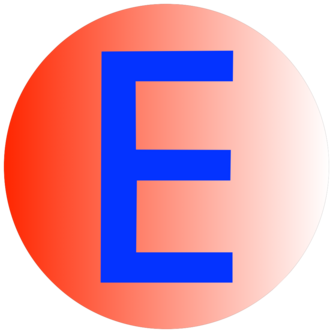
\includegraphics[width=4cm]{eicon333.png}\\[5ex]E 3.1\\[1.5ex]User Manual\\[1.5ex]{\normalsize --preliminary
    version--}}

\makeindex{}

\begin{document}
\maketitle{}

\begin{abstract}
  E is an equational theorem prover for full first-order logic and
  monomorphic higher-order logic, based on superposition and
  rewriting. In this perpetually preliminary manual we first give a
  short introduction and basic usage information for new users, and
  then cover calculus and proof procedure. The manual also covers
  proof search control and related options, followed by input and
  output formats. Finally, it describes some additional tools that are
  part of the E distribution.
\end{abstract}

\tableofcontents{}

\chapter{Introduction}
\label{sec:intro}

This is a short and currently quite sketchy documentation of the
equational theorem prover E. E is an purely equational theorem prover
for full first-order logic with equality, and, as of E~3.0, for
monomorphic higher-order logic. It is based on paramodulation and
rewriting. This means that E reads a set of formulas and/or clauses
and saturates it by systematically applying a number of inference
rules until either all possible (non-redundant) inferences have been
performed or until the empty clause has been derived, i.e.\ the clause
set has been found to be unsatisfiable and thus the conjecture has
been proved.

Even after 20 years, E is still a moving target. However, most recent
releases have been quite stable, and the prover is being used
productively by several independent groups of people. This manual
should enable you to experiment with the prover and to use some of its
more advanced features. Be aware that it often lags behind the
implementation. The ultimate reference is the source code. Also, the
help page (produced \texttt{eprover -h} and equivalent to the UNIX man
page delivered with the prover) is always an up-to-date documentation
of the available command line options

The manual assumes a working knowledge of refutational theorem
proving, which can be gained from e.g.~\cite{CL73}. The calculus is
(mostly) a specialisation of superposition as described by Bachmair
and Ganzinger~\cite{BG94}.

The primary description of E has been published
as~\cite{Schulz:AICOM-2002}, while the most recent published
descriptions are~\cite{Schulz:LPAR-2013} (including the extension to
many-sorted logic) and~\cite{SCV:CADE-2019} (including optional
extension to LFHO and integration of PicoSAT). A more extensive
description of the LFHO extension can be found
in~\cite{VBCS:TACAS-2019,VBCS:STTT-2021}. Extensions to full higher
order logic are covered in~\cite{VBS:TACAS-2023}. Most papers on E and
much more information is available at or a few hops away from the E
home page, \url{https://www.eprover.org}.

Some other provers have influenced the design of E and may be
referenced in the course of this manual. These include
SETHEO\index{SETHEO}~\cite{MILSGSM:JAR-97},
Otter\index{Otter}~\cite{Mc94,MW:JAR-97},
SPASS\index{SPASS}~\cite{WGR96,WABCEKTT:CADE-99},
DISCOUNT~\cite{DKS97}, Waldmeister~\cite{BHF96,HJL:CADE-99} and
Vampire\index{Vampire}~\cite{RV:AICOM-2002,RV:IJCAR-2001,KV:CAV-2013}.


\chapter{Getting Started}
\label{sec:start}

Installation of E should be straightforward, but requires a standard
UNIX/Linux build environment, including \texttt{/bin/sh}, \texttt{gcc}
(or an equivalent compiler), and \texttt{make}. The file
\texttt{README} (or, somewhat nicer, \texttt{README.md}) in the main
directory of the distribution contains the necessary
information. After configuring and building the system, you will find
the stand-alone executable \texttt{E/PROVER/eprover}, or
\texttt{E/PROVER/eprover-ho} if you configured the system with support
for higher-order logic.

E is controlled by a very wide range of parameters. However, if you do
not want to bother with the details, you can leave configuration for a
problem to the prover. To use this feature, use the following command
line options:

\bigskip
\noindent
\begin{tabular}{lp{7.5cm}}
  \texttt{--satauto}
  & Choose literal selection strategy,  clause
    evaluation heuristic, term ordering and other search parameters
    automagically\index{xyzzy}, based on problem features.\\
  \texttt{--auto}
  & As \texttt{--satauto}, but add heuristic
    specification pruning using one of several instantiation of the SInE
    algorithm~\cite{HV:CADE-2011} for large specifications. This makes
    the prover potentially incomplete.\\
  \texttt{--auto-schedule}
  & As \texttt{--auto}, but try not one, but
    several different strategies. \\
  \texttt{--memory-limit=xx}
  & Tell the prover how much memory
    (measured in MB) to use at most. In automatic mode E will optimize
    its behaviour for this amount (32~MB will work, 128~MB is
    reasonable, 1024~MB is what I use. \emph{More is
    better}\footnotemark, but if you go over
    your physical memory, you will probably experience \emph{very} heavy
    swapping.) Due to limitations of \texttt{rlim\_t}, values over 2047
    may not work on all platforms. If you have ab up-to-date machine
    and plan on running the prover for a few minutes at most, this has
    become a lot less critical than in the past.\\
\end{tabular}
\footnotetext{Emphasis added for E~0.7 and up, which globally cache
  rewrite steps.}

\begin{example}
  If you happen to have a workstation with 64 MB RAM\footnote{Yes,
    this is outdated. If it still applies to you, get a new
    computer! It will still work ok, though.}, the following command
  is reasonable:\nopagebreak
\small\nopagebreak
\begin{verbatim}
eprover --auto --memory-limit=48 PUZ031-1+rm_eq_rstfp.lop
\end{verbatim}
  \normalsize
\end{example}



\chapter{Calculus and Proof Procedure}
\label{sec:calculus}

E is a purely equational theorem prover, based on ordered
paramodulation and rewriting. As such, it implements an instance of
the superposition calculus described in~\cite{BG94}. We have added
some stronger contraction rules and a more general approach to literal
selection, and have also extended the calculus to simple, monomorphic
many-sorted logic (in the sense of the TPTP-3 TFF
format~\cite{SSCB:LPAR-2012}).

The core proof procedure is a variant of the \emph{given-clause}
algorithm. However, before proof search in clause normal form (CNF)
begins, various transformations can be applied to the input
problem. In particular, E processes not only clausal problems, but can
read full first order format, including a rich set of formula roles,
logical operators and quantifiers. This format is reduced to clause
normal form in a way that the CNF is unsatisfiable if and only if the
original problem is provable (if an explicit \emph{conjecture} is
given) or itself unsatisfiable.


\section{Calculus}

We assume a finite set $S=\{S_i\}$ of \emph{sorts}\index{sort}
(or atomic types), with each sort interpreted by a non-empty domain
disjoint from the domains of all other sorts. With each sort $S_i$ we
associate an enumerable set of variables\index{variable} $V_{S_i}$, with
$V_S\cap V_T = \emptyset$ if $S\not=T$ (i.e.\ each variable has a
unique sort). We assume at least two sorts, \texttt{\$i} (individuals)
and \texttt{\$o} (truth values).

A \emph{type}\index{type} is a non-empty tuple $(S_1, \ldots, S_n, T)$
with $T\in S$ and $S_i \in S$ for all $S_i$. We usually write a type
as $(S_1, \ldots, S_n) \to T$. The $S_i$ are called \emph{argument
  sorts} and $T$ is called the \emph{resulting sort}.

A signature $F$ is a finite set of function symbols with associated
types. We write $f:(S_1, \ldots, S_n)
 \to T$ to indicate that $f$ is
of type $(S_1, \ldots, S_n) \to T$.

\emph{Term}$(F,V)$\index{term} denotes the set of (sorted first order)
\emph{terms} over \emph{F} and \emph{V}, defined as follows:
$x \in V_{S_i}$ is a term of sort $S_i$. If
$f:(S_1, \ldots, S_n) \to T$ is a function symbol in $F$ and
$t_1, \ldots t_n$ are terms of sorts $S_1, \ldots S_n$, respectively,
then $f(s_1, \ldots, s_n)$ is a term of sort $T$. We require that the
$S_i\not=\mathtt{\$o}$, and call function symbols with resulting type
\texttt{\$o} \emph{predicate symbols}.

We write $t|_p$ to denote the subterm\index{subterm} of $t$ at a
position $p$ and write $t[p\leftarrow t']$ to denote $t$ with $t|_p$
replaced by $t'$. An equation\index{equation} \eqn{s}{t} is an
(implicitly symmetrical) pair of terms (of the same sort). A positive
literal\index{literal} is an equation \eqn{s}{t}, a negative literal
is a negated equation \neqn{s}{t}.  We write \ueqn{s}{t} to denote an
arbitrary literal.\footnote{Non-equational literals are encoded as
  equations or disequations \ueqn{P(t_1, \ldots, t_n)}{\top}, where
  the resulting sort of $P$ and $\top$ is \texttt{\$o}.

  In other words, we treat predicate symbols as special function
  symbols that can only occur at the top-most positions and demand
  that atoms (terms formed with a top predicate symbol) cannot be
  unified with a first-order variable, i.e.\ we treat normal terms and
  predicate terms as disjoint sorts. We sometimes write the literal
  $\eqn{P(t_1, \ldots, t_n)}{\top}$ as $P(t_1, \ldots, t_n)$ and
  $\neqn{P(t_1, \ldots, t_n)}{\top}$ as $\neg P(t_1, \ldots, t_n)$ for
  simplicity.} Literals can be represented as multi-sets of multi-sets
of terms, with \eqn{s}{t} represented as $\{\{s\},\{t\}\}$ and
\neqn{s}{t} represented as $\{\{s, t\}\}$.  A \emph{ground reduction
  ordering}\index{ordering}\index{reduction ordering} $>$ is a
Noetherian partial ordering that is stable w.r.t. the term structure
and substitutions and total on ground terms. $>$ can be extended to an
ordering $>_L$ on literals by comparing the multi-set representation
of literals with $>\!\!> >\!\!>$ (the multi-set-multi-set extension of
$>$).

Clauses are multi-sets of literals. They are usually represented as
disjunctions of literals, $\ueqn{s_1}{t_1} \vee \ueqn{s_2}{t_2} \ldots
\vee \ueqn{s_n}{t_n}$. We write \mw{Clauses(F,P,V)} to denote the set
of all clauses with function symbols $F$, predicate symbols $P$ and
variables $V$. If $\mathcal{C}$ is a clause, we denote the (multi-)set
of positive literals in $\mathcal{C}$ by $\mathcal{C^+}$ and the
(multi-)set of negative literals in $\mathcal{C}$ by $\mathcal{C^-}$
We extend $>_L$ to clauses by defining $>_C = >_L>_L$, i.e.\ we
compare clauses as multi-sets of literals.

We write $s[t\leftarrow t']$ to denote the term $s$ in which every
occurrence of the subterm $t$ has been replaced by $t'$. We extend this
notion to literals and clauses (i.e.\ $C[t\leftarrow t']$ is the
clause $C$ in which all occurrences of $t$ have been replaced by
$t'$).

A \emph{substitution}\index{substitution} is a function
$\sigma: V\to \mw{Term}(F,V)$ with the properties that
$|\{ x\in V \mid \sigma(x)\not=x\}| \in \nat$ (i.e.\ only finitely
many variables are substituted) and that $x$ and $\sigma(x)$ are terms
of the same sort for all $x \in V$. Substitutions are extended to
literals and clauses in the obvious way. A \emph{most general
  unifier}\index{mgu}\index{most general unifier} of two terms $s$ and
$t$ is a substitution $\sigma$ with $\sigma(s)=\sigma(t)$ and with the
property that no other unifier is more general than $\sigma$. If the
\emph{mgu} of two terms exists, it is unique up to variable renaming,
so we usually speak of \emph{the} most general unifier of two terms
and denote it by $\mw{mgu}(s,t)$.

In the following, most inferences between clauses are performed at
particular literals of the clauses. Inference literals can be
determined the term ordering, or, sometimes, by \emph{selection}.  The
introduction of an extended notion of \emph{literal selection} has
improved the performance of E significantly. The necessary concepts
are explained in the following.

\begin{definition}[Selection functions]
  \label{def:basics:inferences:selection}
  \index{selection functions}
  $\mw{sel}:\mw{Clauses(F,P,V)} \rightarrow \mw{Clauses(F,P,V)}$ is a
  \emph{selection function}, if it has the following properties for
  all clauses $\mathcal{C}$:
    \begin{itemize}
    \item $\mw{sel}(\mathcal{C}) \subseteq \mathcal{C}$.
    \item If $\mw{sel}(\mathcal{C})\cap \mathcal{C^-} = \emptyset$, then
      $\mw{sel}(\mathcal{C}) = \emptyset$.
    \end{itemize}
    We say that a literal $\mathcal{L}$ is \emph{selected} (with
    respect to a given selection function) in a clause $\mathcal{C}$
    if $\mathcal{L} \in \mw{sel}(\mathcal{C})$.
  \hfill$\blacktriangleleft$
\end{definition}

We will use two kinds of restrictions on deducing new clauses: One
induced by ordering constraints and the other by selection functions.
We combine these in the notion of \emph{eligible literals}.

\begin{definition}[Eligible literals]
  \index{literal!eligible}
  \index{eligible for paramodulation|see{literal, eligible}}
  \index{eligible for resolution|see{literal, eligible}}
  \index{eligible literals|see{literal, eligible}}
 \label{def:basics:inferences:eligible}
 Let $\mathcal{C} = \mathcal{L} \vee \mathcal{R}$ be a clause, let
 $\sigma$ be a substitution and let $\mw{sel}$ be a selection
 function.
 \begin{itemize}
 \item We say $\sigma(\mathcal{L})$ is \emph{eligible for
     resolution} if either
   \begin{itemize}
   \item $\mw{sel}(\mathcal{C}) = \emptyset$ and $\sigma(\mathcal{L})$
     is $>_L$-maximal in $\sigma(\mathcal{C})$ or
   \item $\mw{sel}(\mathcal{C}) \not= \emptyset$ and
     $\sigma(\mathcal{L})$ is $>_L$-maximal in
     $\sigma(\mw{sel}(\mathcal{C})\cap \mathcal{C^-})$ or
   \item $\mw{sel}(\mathcal{C}) \not= \emptyset$ and
     $\sigma(\mathcal{L})$ is $>_L$-maximal in
     $\sigma(\mw{sel}(\mathcal{C})\cap \mathcal{C^+})$.
   \end{itemize}
 \item $\sigma(\mathcal{L})$ is \emph{eligible for paramodulation} if
   $\mathcal{L}$ is positive, $\mw{sel}(\mathcal{C}) = \emptyset$ and
   $\sigma(\mathcal{L})$ is strictly $>_L$-maximal in
   $\sigma(\mathcal{C})$.
 \end{itemize}
 \hfill$\blacktriangleleft$
 \index{literal!eligible}
\end{definition}


The calculus is represented in the form of inference rules. For
convenience, we distinguish two types of inference rules. For
\emph{generating} inference rules, written with a single line
separating preconditions and results, the result is added to the set
of all clauses. For \emph{contracting} inference rules, written with a
double line, the result clauses are substituted for the clauses in the
precondition. In the following, $u$, $v$, $s$ and $t$ are terms,
$\sigma$ is a substitution and $R$, $S$ and $T$ are (partial) clauses.
$p$ is a position in a term and $\lambda$ is the empty or
top-position. $D \subseteq F$ is a set of unused constant predicate
symbols. Different clauses are assumed to not share any common
variables.


\begin{definition}[The inference system \textbf{SP}]
 \label{def:basics:inferences:sp}\index{SP@\textbf{SP} (calculus)}
 Let $>$ be a total simplification ordering (extended to orderings
 $>_L$ and $>_C$ on literals and clauses), let $\mw{sel}$ be a
 selection function, and let $D$ be a set of fresh propositional
 constants. The inference system \textbf{SP} consists of the following
 inference rules:

 \begin{itemize}
 \item \emph{Equality Resolution}\index{equality resolution}:

   \bigskip (ER) \GInferenz{\neqn{u}{v} \vee R}{\sigma(R)}{if
     $\sigma{} = \mw{mgu}(u,v)$ and $\sigma(\neqn{u}{v})$ is eligible
     for resolution.}

 \item \emph{Superposition into negative
     literals}\index{superposition!inference rule}:

   \bigskip (SN) \GInferenz{\eqn{s}{t} \vee S \phantom{ae}
     \neqn{u}{v} \vee R}{\sigma(\neqn{u[p\leftarrow t]}{v} \vee S
     \vee R)}{if $\sigma=mgu(u|_p,s)$, $\sigma(s)\not<\sigma(t)$,
     $\sigma(u)\not<\sigma(v)$, $\sigma(\eqn{s}{t})$ is eligible for
     paramodulation, $\sigma(\neqn{u}{v})$ is eligible for resolution,
     and $u|_p \notin V$.}

 \item \emph{Superposition into positive
     literals}\index{superposition!inference rule}:

   \bigskip (SP) \GInferenz{\eqn{s}{t} \vee S \phantom{ae}
     \eqn{u}{v} \vee R}{\sigma(\eqn{u[p\leftarrow t]}{v} \vee S \vee
     R)}{if $\sigma=mgu(u|_p,s)$, $\sigma(s)\not<\sigma(t)$,
     $\sigma(u)\not<\sigma(v)$, $\sigma(\eqn{s}{t})$ is eligible for
     paramodulation, $\sigma(\eqn{u}{v})$ is eligible for
     resolution, and $u|_p \notin V$.}


 \item \emph{Simultaneous superposition into negative
     literals}\index{simultaneous superposition}

    \bigskip (SSN) \GInferenz{\eqn{s}{t} \vee S \phantom{ae} \neqn{u}{v} \vee
     R}{\sigma(S \vee (\neqn{u}{v} \vee R)[u|_p\leftarrow{}t])}{if
     $\sigma=mgu(u|_p,s)$, $\sigma(s)\not<\sigma(t)$,
     $\sigma(u)\not<\sigma(v)$, $\sigma(\eqn{s}{t})$ is eligible for
     paramodulation, $\sigma(\neqn{u}{v})$ is eligible for resolution,
     and $u|_p \notin V$.}

   This inference rule is an alternative to (SN). Note that the
   difference is that \emph{every} occurrence of the subterm unified
   with the right-hand side of the rewriting clause is replaced by the
   (instance of) the left hand side in the (instance of) the clause
   that is rewritten. This single rule usually performs better than a
   sequence of conventional superpositions in practice.

\item \emph{Simultaneous superposition into positive literals}
  \index{simultaneous superposition}

  \bigskip (SSP) \GInferenz{\eqn{s}{t} \vee S \phantom{ae} \eqn{u}{v}
    \vee R}{\sigma(S \vee (\eqn{u}{v} \vee R)[u|_p\leftarrow
    t])}{if $\sigma=mgu(u|_p,s)$, $\sigma(s)\not<\sigma(t)$,
    $\sigma(u)\not<\sigma(v)$, $\sigma(\eqn{s}{t})$ is eligible for
    paramodulation, $\sigma(\neqn{u}{v})$ is eligible for resolution,
    and $u|_p \notin V$.}

  This inference rule is an alternative to (SP) that performs better
  in practice. See the note on the previous rule.

 \item \emph{Equality factoring}\index{equality factoring}:

   \bigskip (EF) \GInferenz{\eqn{s}{t} \vee \eqn{u}{v} \vee
     R}{\sigma(\neqn{t}{v} \vee \eqn{u}{v} \vee R)}{if
     $\sigma=mgu(s,u)$, $\sigma(t) \not> \sigma(s)$ and
     $\sigma(\eqn{s}{t})$ eligible for paramodulation.}


 \item \emph{Rewriting of negative literals}\index{rewriting}:

   \bigskip (RN) \CInferenz{\eqn{s}{t} \phantom{ae}
     \neqn{u}{v} \vee R} {\eqn{s}{t}
     \phantom{ae} \neqn{u[p\leftarrow{} \sigma(t)]}{v} \vee R} {if
     $u|_p = \sigma(s)$ and $\sigma(s)>\sigma(t)$.}


 \item \emph{Rewriting of positive
     literals}\index{rewriting}\footnote{A stronger version of (RP)
     is proven to maintain completeness for Unit and Horn problems
     and is generally believed to maintain completeness for the
     general case as well~\cite{Bachmair:personal-98}.  However, the
     proof of completeness for the general case seems to be rather
     involved, as it requires a very different clause ordering than
     the one introduced~\cite{BG94}, and we are not aware of any
     existing proof in the literature. The variant rule allows
     rewriting of maximal terms of maximal literals under certain
     circumstances:

     \medskip
     (RP') \CInferenzFoot{\eqn{s}{t} \phantom{ae}
       \eqn{u}{v} \vee R} {\eqn{s}{t}
       \phantom{ae} \eqn{u[p\leftarrow{} \sigma(t)]}{v} \vee R} {if
       $u|_p = \sigma(s)$, $\sigma(s)>\sigma(t)$ and
       if \eqn{u}{v} is not eligible for
       paramdulation or $u \not> v$ or $p \not=
       \lambda$ or $\sigma$ is not a variable renaming.}

     \medskip \noindent This stronger rule is implemented successfully
     by both E\index{E (theorem prover)} and
     SPASS\index{SPASS}~\cite{Weidenbach:personal-99}.}:

   \bigskip (RP) \CInferenz{\eqn{s}{t} \phantom{ae} \eqn{u}{v} \vee R}
   {\eqn{s}{t} \phantom{ae} \eqn{u[p\leftarrow{} \sigma(t)]}{v} \vee
     R} {if $u|_p = \sigma(s)$, $\sigma(s)>\sigma(t)$, and if
     \eqn{u}{v} is not eligible for paramodulation or $v > u$ or $p
     \not= \lambda$.}

 \item \emph{Clause subsumption}\index{subsumption}:

   \bigskip (CS) \CInferenz{C \phantom{ae} \sigma(C \vee R)}{C}{where
     $C$ and $R$ are arbitrary (partial) clauses and $\sigma$ is a
     substitution.}

 \item \emph{Equality subsumption}\index{subsumption}:

   \bigskip (ES) \CInferenz{\eqn{s}{t} \phantom{ae}
     \eqn{u[p\leftarrow{} \sigma(s)]}{u[p\leftarrow{}
       \sigma(t)]\vee R}}{\eqn{s}{t}}{}

 \item \emph{Positive simplify-reflect\index{simplify-reflect}\footnote{In
       practice, this rule is only applied if $\sigma(s)$ and
       $\sigma(t)$ are $>$-incomparable -- in all other cases this
       rule is subsumed by (RN) and the deletion of resolved literals
       (DR).}}:

   \bigskip (PS) \CInferenz{\eqn{s}{t} \phantom{ae}
     \neqn{u[p\leftarrow{} \sigma(s)]}{u[p\leftarrow{}
       \sigma(t)]\vee R}}{\eqn{s}{t} \phantom{aee} R}{}


 \item \emph{Negative simplify-reflect\index{simplify-reflect}}

   \bigskip (NS) \CInferenz{\neqn{s}{t} \phantom{ae}
     \neqn{\sigma(s)}{\sigma(t)\vee R}}{\neqn{s}{t} \phantom{aee} R}{}

% \item \emph{Contextual (top level) simplify-reflect\index{contextual
%       simplify-reflect}}
%
%   \bigskip (CSR) \CInferenz{\sigma(C \vee R \vee \doteqn{s}{t})
%     \hspace{2em} C \vee \overline{\doteqn{s}{t}}}{\sigma(C \vee R)
%     \hspace{5em} C \vee \overline{\doteqn{s}{t}}}
%   {where $\overline{\doteqn{s}{t}}$ is the negation of $\doteqn{s}{t}$
%     and $\sigma$ is a substitution}


 \item \emph{Tautology deletion}\index{tautology deletion}:

   \bigskip (TD) \CInferenz{C}{}{if C is a tautology\footnotemark{}}
   \footnotetext{This rule can only be implemented approximately, as
     the problem of recognizing tautologies is only semi-decidable in
     equational logic. Current versions of
     E try to detect tautologies by checking if the ground-completed
     negative literals imply at least one of the positive literals, as
     suggested in~\cite{NN:RTA-93}.}

 \item \emph{Deletion of duplicate literals}:

   \bigskip (DD) \CInferenz{\eqn{s}{t} \vee \eqn{s}{t} \vee
     R}{\eqn{s}{t} \vee R}{}

 \item \emph{Deletion of resolved literals}:

   \bigskip (DR) \CInferenz{\neqn{s}{s} \vee R}{R}{}

 \item \emph{Destructive equality resolution}\index{equality
     resolution}:

   \bigskip (DE) \CInferenz{\neqn{x}{y} \vee R}{\sigma(R)}{if $x,y \in
     V, \sigma = mgu(x,y)$}

 \item \emph{Contextual literal cutting}\index{contextual literal
     cutting}:

   \bigskip (CLC) \CInferenz{\sigma(C \vee R \vee
     \ueqn{s}{t}) \hspace{2em} C \vee \overline{\ueqn{s}{t}}}{\sigma(C
     \vee R) \hspace{5em} C \vee \overline{\ueqn{s}{t}}} {where
     $\overline{\ueqn{s}{t}}$ is the negation of $\ueqn{s}{t}$ and
     $\sigma$ is a substitution}

   This rule is also known as \emph{subsumption resolution} or
   \emph{clausal simplification}.


\item \emph{Condensing}\index{condensing}:

   \bigskip (CON) \CInferenz{l_1 \vee l_2 \vee R}{\sigma(l_1 \vee R)}{if
  $\sigma(l_1) = \sigma(l_2)$ and $\sigma(l_1 \vee R)$ subsumes
  $l_1 \vee l_2 \vee R$}



 \item \emph{Introduce definition\index{clause
       splitting}}\footnote{This rule is always exhaustively applied to
     any clause, leaving n split-off clauses and one final link clause of
     all negative propositions.}

   \bigskip (ID) \CInferenz{R \vee S}{d \vee R \phantom{ae} \neg d \vee
     S}{if $R$ and $S$ do not share any variables, $d \in D$ has not
     been used in a previous definition and $R$ does not contain any
     symbol from $D$}

 \item \emph{Apply definition\index{clause splitting}}

   \bigskip (AD) \CInferenz{\sigma (d \vee R) \phantom{ae} R \vee S}
   {\sigma(d \vee R) \phantom{ae} \neg d \vee S}{if $\sigma$ is a
     variable renaming, $R$ and $S$ do not share
     any variables, $d \in D$ and $R$ does not contain any symbol from
     $D$}


 \end{itemize}
 We write $\mathbf{SP}(N)$ to denote the set of all clauses that can
 be generated with one generating inference from $\mathbf{SP}$ on a
 set of clauses $N$, $\mathcal{D}_{SP}$ to denote the set of all
 \textbf{SP}-derivations, and $\mathcal{D}_{\overline{SP}}$ to denote
 the set of all finite \textbf{SP}-derivations.

  \hfill$\blacktriangleleft$
\end{definition}



As \textbf{SP} only removes clauses that are \emph{composite} with
respect to the remaining set of clauses, the calculus is complete. For
the case of unit clauses, it degenerates into \emph{unfailing}
completion~\cite{BDP89} as implemented in DISCOUNT\index{DISCOUNT}. E
can also simulate the positive unit strategy for Horn clauses
described in~\cite{Dershowitz:IJCAI-91} using appropriate selection
functions.

Contrary to e.g.\ SPASS\index{SPASS}, E does not implement special
rules for non-equa\-tio\-nal literals or sort theories. Non-equational
literals are encoded as equations and dealt with accordingly.


\section{Preprocessing}

\subsubsection{Axiom Filtering}
\label{:secsine}

Real-life axiom sets have grown steadily over the last years. One
increasing application for deduction is e.g. the answering of questions
based on large common-sense ontologies. Such specifications can
contain from several thousand to several million input axioms, only a
small part of which are necessary for any given query.

To avoid swamping the inference engine with most likely irrelevant
facts, E implements two different filtering mechanisms. Both start
with the conjecture, select facts that are likely connected to the
conjecture, and then recursively apply this process again.

\begin{itemize}
\item Classical \emph{relevancy pruning}\index{relevancy pruning}
  starts with the function and predicate symbols in the goal. Every
  axiom that shares such a symbol is considered relevant. Symbols in
  relevant axioms become relevant themselves. The process is then
  repeated for a selected number of iterations. The option
  \texttt{--rel-pruning-level} determines how many iterations are
  performed.  Relevance pruning is complete in the non-equational case
  if allowed to reach a fixed point. It only provides a relatively
  coarse measure, however.
\item More fine-grained control is offered by the SInE\index{SInE}
  method~\cite{HV:CADE-2011}. SInE does not consider \emph{all}
  symbols in already selected clauses and formulas to be relevant, but
  defines a \emph{D-relation} that determines which symbols to
  consider relevant. E implements a frequency-based D-relation: in
  every clause or formula, the least frequently occurring symbols are
  considered relevant.

  SInE in E is controlled via the option \texttt{--sine}. It takes as
  its argument either the name of a predefined SInE filter
  specification, or a newly defined strategy. The default is
  equivalent to \texttt{--sine=Auto} and will automatically determine
  if axiom filtering should be applied, and if yes, which filter
  should be applied. Filter selection is based on a number of features
  of the problem specification, and on performance of different
  filters on the TPTP\index{TPTP} problem library.

  A SInE-Filter for E is specified as follows:
\begin{verbatim}
<sine-filter> ::= GSinE(<g-measure>,
                        hypos|nohypos,
                        <benvolvence>,
                        <generosity>,
                        <rec-depth>,
                        <set-size>,
                        <set-fraction> [,
                        addnosymb|ignorenosymb])
\end{verbatim}
  \begin{itemize}
  \item \texttt{<g-measure>} is the generality measure. Currently,
    \texttt{CountFormulas} and \texttt{CountTerms} are supported. The
    first considers a symbol more general than another if it occurse
    in more formulas. The second counts the number of subterms which
    contain the symbol as the top symbol.
  \item \texttt{hypos} or \texttt{nohypos} determines if clauses and
    formulas of type \texttt{hy\-po\-the\-sis} are used as additional seeds
    for the analysis.
  \item \texttt{<benevolence>} is a floating point value that determines
    how much more general a function symbol in a clause or formula is
    allowed to be relative to the least general one to be still
    considered for the D-relation.
  \item \texttt{<generosity>} is an integer count and determines how
    many symbols are maximally considered for the D-relation of each
    clause or formula.
  \item \texttt{<rec-depth>} determines the maximal number of
    iterations of the selection algorithm.
  \item \texttt{<set-size>} gives an absolute upper bound for the
    number of clauses and formulas selected.
  \item \texttt{set-fraction} gives a relative size (which fraction
    of clauses/formulas) will be at most selected
  \item Finally, the optional last argument determines if clauses or
    formulas which do not contain any function- or predicate symbols
    pass the filter. This is a rare occurence, so the effect is minor
    in either case.
  \end{itemize}
\end{itemize}

\subsubsection{Clausification}
\label{sec:cnf}

E converts problems in full FOF into clause normal form using a
slightly simplified version of the algorithm described by Nonnengart
and Weidenbach~\cite{NW:SmallCNF-2001}\index{clausification}. E's
algorithm has the following modifications:
\begin{itemize}
\item E supports the full set of first-order connectives defined in
  the TPTP-3 language\index{TPTP!language}.
\item E is more eager about introducing definitions to keep the CNF
  from exponential explosion. E will introduce a definition for a
  sub-formula, if it can determine that it will be duplicated more than
  a given number of times in the naive output. The limit can be set
  with the option \texttt{--definitional-cnf}. E will reuse
  definitions generated for one input formula for syntactically
  identical formulae in other formulas with the same specification.
\item E supports mini-scoping, but not the more advanced forms of
  Skolemization.
\end{itemize}

It is possible to use E as a clausifier only. When given the
\texttt{--cnf} option, E will just perform clausification and print
the resulting clause set.


\subsubsection{Equational Definition unfolding}\index{equational definition}
\label{sec:eqdef}

Equational definitions are unit clauses of the form $f(X_1, \ldots,
X_n)=t$, where $f$ does not occur in $t$, and all variables in $t$ are
also in $f$. In this case, we can completely replace all occurrences of
$f$ by the properly instantiated $t$. This reduces the size of the
search space, but can increase the size of the input specification. In
particular in the case of nested occurrences of $f$, this increase can
be significant.

E controls equational definition unfolding with the following options:

\texttt{--eq-unfold-limit=<arg>} limits unfolding (and removing) of
equational definitions to those where the expanded definition is at
most the given limit bigger (in terms of standard term weight) than
the defined term.

\texttt{--eq-unfold-maxclauses=<arg>} inhibits  unfolding of
equational definitions if the problem has more than the stated limit
of clauses.

\texttt{--no-eq-unfolding} disables equational definition unfolding
completely.



\subsubsection{Presaturation Interreduction}
\label{sec:presat}

If the option \texttt{--presat-simplify} is set, E will perform an
inital interreduction\index{interreduction} of the clause set. It will
exhaustively apply simplifying inferences by running its main proof
procedure while disabling generating inferences.

Some problems can be solved purely by simplification, without the need
for deducing new clauses via the expensive application of the
generating inference rules, in particularly
paramodulation/superposition. Moreover, exhaustive application of
simplifying inferences can reduce redundancy in the specification and
allows all input clauses to be evaluated under the same initial
conditions. On the down side, a complete interreduction of the input
problem can take significant time, especially for large
specifications.



\section{Proof Procedure}
\label{sec:procedure}

\begin{figure}[hp]
  \begin{center}
    \tt
    \begin{tabbing}
      \quad\quad \= \quad\quad \= \quad\quad \=  \quad\quad \= \quad\quad \= \kill
      \# Input: Axioms in U, P is empty\\
      while U $\not= \emptyset{}$ begin\+\\
         \# First check for propositional unsat (Section \ref{sec:cdcl})\\
         if \text{prop\_trigger}(U,P)\+\\
            if \text{prop\_unsat\_check}(U,P)\+\\
                 SUCCESS, Proof found\-\-\\
        c := select(U)\\
        U := U $\backslash$ \{c\}\\

        \# Apply (RN), (RP), (NS), (PS), (CLC), (DR), (DD), (DE)\\
        simplify(c,P)\\
        \# Apply (CS), (ES), (TD)\\
        if c is trivial or subsumed by P then\+\\
          \# Delete/ignore c\-\\
        else if c is the empty clause then\+\\
          \# Success: Proof found\\
          stop\-\\
        else\+\\
          T := $\emptyset{}$ \# Temporary clause set\\
          foreach p $\in$ P do\+\\
            if p can be simplified with c \+\\
              P := P $\backslash$ \{p\}\\
              U := U $\backslash$ \{d|d \mbox{ is direct descendant of } p\}\\

              T := T $\cup$ \{p\}\-\\
            done\-\\
          end\\
          P := P $\cup$ \{c\}\\
          T := T $\cup$ e-resolvents(c)    \# (ER)\\
          T := T $\cup$ e-factors(c)       \# (EF)\\
          T := T $\cup$ paramodulants(c,P) \# (SN), (SP)\\
          T' := \{\}\\
          foreach p $\in$ T do\+\\
            \# Apply efficiently implemented subset of (RN),\\
            \# (RP), (NS), (PS), (CLC), (DR), (DD), (DE)\\
            p := cheap\_simplify(p, P)\\
            \# Apply (TD) or efficient approximation of it\\
            if p is trivial\+\\
              \# Delete/ignore p\-\\
            else\+\\
               T' := T' $\cup$ cheap\_simplify(p, P)\-\\
            fi\-\\
          end\\
          U := U $\cup$ T' \-\\
        fi\-\\
      end\\
      \# Failure: Initial U is satisfiable, P describes model
    \end{tabbing}
    \normalfont
    \caption{Main proof procedure of E}
    \label{fig:procedure}\index{proof procedure}
  \end{center}
\end{figure}

Fig.~\ref{fig:procedure} shows a (slightly simplified) pseudocode
sketch of the quite straightforward proof procedure of E. The set of
all clauses is split into two sets, a set \texttt{P} of
\emph{processed} clauses and a set \texttt{U} of \emph{unprocessed}
clauses. Initially, all input clauses are in in \texttt{U}, and
\texttt{P} is empty. In its normal mode of operation, at each
iteration of the look the algorithm selects a new clause (sometimes
called the \emph{given clause}\index{given clause}) from \texttt{U},
simplifies it w.r.t. to \texttt{P}, then uses it to back-simplify the
clauses in \texttt{P} in turn. It then performs equality factoring,
equality resolution and superposition between the selected clause and
the set of processed clauses. The generated clauses are simplified and
added to the set of unprocessed clauses. The process stops when the
empty clause is derived or no further inferences are possible.

The proof search is controlled by three major parameters: The term
ordering (described in section~\ref{sec:options:orderings}), the
literal selection function, and the order in which the \texttt{select}
operation selects the next \emph{given clause} to process.

E implements two different classes of term orderings\index{term
  ordering}, lexicographic term orderings and Knuth-Bendix
orderings. A given ordering is determined by instantiating one of the
classes with a variety of parameters (described in
section~\ref{sec:options:orderings}).

Literal selection\index{literal!selection} currently is done according
to one of more than 50 predefined
functions. Section~\ref{sec:options:strategies} describes this
feature.

Clause selection is determined by a heuristic evaluation function,
which conceptually sets up a set of priority queues and a weighted
round robin scheme that determines from which queue the next clause is
to be picked. The order within each queue is determined by a priority
function (which partitions the set of unprocessed clauses into one or
more subsets) and a heuristic evaluation function, which assigns a
numerical rating to each clause.  Section~\ref{sec:options:heuristics}
describes the user interface to this mechanism.


\subsection{Propositional Reasoning}
\label{sec:cdcl}

As of E 2.1, and with a more refined implementation in E 2.2, the
prover supports efficient propositional reasoning\index{propositional
  reasoning} by integrating
PicoSAT\index{PicoSAT}~\cite{Biere:JSBC-2008}. The prover periodically
grounds all clauses in the proof state and encodes the set of ground
clauses for the propositional solver. If the propositional solver
finds a proof for unsatisfiability of the ground problem, Herbrand's
theorem allow us to lift this to the first-order level. In the
implementation, the prover extract the unsatisfiable core of the
grounded clause set, retrieves the corresponding first-order clauses,
and adds an suitable pseudo-inference to the first-order proof
objects. A more detailed description is available
in~\cite{Schulz:Vampire-2018}.

See section~\ref{sec:cdclopt} for options controlling this feature.

\chapter{Controlling the Proof Search}
\label{sec:options}

This section describes some of the different options available to
control the search of the main proof procedure. The three most
important choice points in the proof search are the choice of
\emph{term ordering}\index{term ordering}, the selection of the
\emph{given clause}\index{given clause} for any iteration of the main
loop, and the (optional) selection of inference
literals\index{literal!selection}. In addition to these major choice
points, there are a large number of additional selections of lesser,
but not insigificant importance.


\section{Search Control Heuristics}
\label{sec:options:heuristics}

Search control heuristics define the order in which the prover
considers newly generated clauses. A heuristic is defined by a set of
\emph{clause evaluation functions} and a selection scheme which defines
how many clauses are selected according to each evaluation function. A
clause evaluation function consists of a \emph{priority function} and
an instance of a generic \emph{weight function}.

\subsubsection{Priority functions}

Priority functions define a partition on the set of clauses.  A single
clause evaluation consists of a priority (which is the first selection
criteria) and an evaluation. Priorities are usually \emph{not}
suitable to encode heuristic control knowledge, but rather are used to
express certain elements of a search strategy, or to restrict the
effect of heuristic evaluation functions to certain classes of
clauses. It is quite trivial to add a new priority function to E, so
at any time there probably exist a few not yet documented here.

Syntactically, a large subset of currently available priority
functions is described by the following rule:

\begin{verbatim}
<prio-fun> ::= PreferGroundGoals ||
               PreferUnitGroundGoals ||
               PreferGround ||
               PreferNonGround ||
               PreferProcessed ||
               PreferNew ||
               PreferGoals ||
               PreferNonGoals ||
               PreferUnits ||
               PreferNonUnits ||
               PreferHorn ||
               PreferNonHorn ||
               ConstPrio ||
               ByLiteralNumber ||
               ByDerivationDepth ||
               ByDerivationSize ||
               ByNegLitDist ||
               ByGoalDifficulty ||
               SimulateSOS||
               PreferHorn||
               PreferNonHorn||
               PreferUnitAndNonEq||
               DeferNonUnitMaxEq||
               ByCreationDate||
               PreferWatchlist||
               DeferWatchlist
\end{verbatim}

The priority functions are interpreted as follows:

\begin{description}
\item[\texttt{PreferGroundGoals}:] Always prefer ground goals (all
  negative clauses without variables), do not differentiate between
  all other clauses.
\item[\texttt{PreferUnitGroundGoals}:] Prefer unit ground goals.
\item[\texttt{PreferGround}:] Prefer clauses without variables.
\item[\texttt{PreferNonGround}:] Prefer clauses with variables.
\item[\texttt{PreferProcessed}:] Prefer clauses that have already been
  processed once and have been eliminated from the set of processed
  clauses due to interreduction (forward contraction).
\item[\texttt{PreferNew}:] Prefer new clauses, i.e. clauses that are
  processed for the first time.
\item[\texttt{PreferGoals}:] Prefer goals (all negative clauses).
\item[\texttt{PreferNonGoals}:] Prefer non goals, i.e. facts with at
  least one positive literal.
\item[\texttt{PreferUnits}:] Prefer unit clauses (clauses with one
  literal).
\item[\texttt{PreferNonUnits}:] Prefer non-unit clauses.
\item[\texttt{PreferHorn}:] Prefer Horn clauses (clauses with no more
  than one positive literals).
\item[\texttt{PreferNonHorn}:] Prefer non-Horn clauses.
\item[\texttt{ConstPrio}:] Assign the same priority to all clauses.
\item[\texttt{ByLiteralNumber}:] Give a priority according to the
  number of literals, i.e. always prefer a clause with fewer literals
  to one with more literals.
\item[\texttt{ByDerivationDepth}:] Prefer clauses which have a short
  derivation depth, i.e. give a priority based on the length of the
  longest path from the clause to an axiom in the derivation
  tree. Counts generating inferences only.
\item[\texttt{ByDerivationSize}:] Prefer clauses which have been
  derived with a small number of (generating) inferences.
\item[\texttt{ByNegLitDist}:] Prefer goals to non-goals. Among goals,
  prefer goals with fewer literals and goals with ground literals
  (more exactly: the priority is increased by 1 for a ground literal
  and by 3 for a non-ground literal. Clauses with lower values are
  selected before clauses with higher values).
\item[\texttt{ByGoalDifficulty}:] Prefer goals to non-goals. Select
  goals based on a simple estimate of their difficulty: First unit
  ground goals, then unit goals, then ground goals, then other goals.
\item[\texttt{SimulateSOS}:] Use the priority system to simulate
  Set-Of-Support. This prefers all initial clauses and all
  Set-Of-Support clauses. Some non-SOS-clauses will be generated, but
  not selected for processing. This is neither well tested nor
  a particularly good fit with E's calculus, but can be used as one
  among many heuristics. If you try a pure SOS strategy, you also
  should set \texttt{--restrict-literal-comparisons} and run the
  prover without literal selection enabled.
\item[\texttt{PreferHorn}:] Prefer Horn clauses (note: includes units).
\item[\texttt{PreferNonHorn}:] Prefer non-Horn clauses.
\item[\texttt{PreferUnitAndNonEq}:] Prefer all unit clauses and all
  clauses without equational literal. This was an attempt to model
  some restricted calculi used e.g.~in Gandalf~\cite{Tammet:JAR-97},
  but did not quite work out.
\item[\texttt{DeferNonUnitMaxEq}:] Prefer everything except for
  non-unit clauses with a maximal equational literal (``Don't
  paramodulate if it is to expensive''). See above, same result.
\item[\texttt{ByCreationDate}:] Return the creation date of the clause
  as priority. This imposes a FIFO equivalence class on
  clauses. Clauses generated from the same given clause are grouped
  together (and can be ordered with any evaluation function among each
  other).
\item[\texttt{PreferWatchlist}] Prefer clauses on the watchlist
  (see~\ref{sec:options:watchlist}).
\item[\texttt{DeferWatchlist}] Defer clauses on the watchlist (see
  above).
\end{description}

Please note that careless use of certain priority functions can make
the prover incomplete for the general case.


\subsubsection{Generic Weight Functions}

Generic weight functions are templates for functions taking a clause
and returning a weight (i.e. an estimate of the usefulness) for it,
where a lower weight means that the corresponding clause should be
processed before a clause with a higher weight.  A generic weight
function is combined with a priority function and instantiated with a
set of parameters to yield a clause evaluation function.

You can specify an instantiated generic weight function as described
in this rule\footnote{Note that there now are many additional generic
  weight functions not yet documented.}:

\small
\begin{verbatim}
<weight-fun> ::= Clauseweight '(' <prio-fun> ', <int>, <int>,
                                  <float> ')'                    ||
                 Refinedweight '(' <prio-fun> ', <int>, <int>,
                                   <float>, <float>, <float> ')' ||
                 Orientweight '(' <prio-fun>, <int>, <int>,
                                  <float>, <float>, <float> ')'  ||
                 Simweight '(' <prio-fun>, <float>, <float>,
                               <float>, <float> ')'              ||
                 FIFOWeight '(' <prio-fun> ')'                   ||
                 LIFOWeight '(' <prio-fun> ')'                   ||
                 FunWeight '(' <prio-fun> ', <int>, <int>,
                               <float>, <float>, <float>
                               (, <fun> : <posint> )* ')'        ||
                 SymOffsetWeight '(' <prio-fun> ', <int>, <int>,
                                     <float>, <float>, <float>
                                    (, <fun> : <int> )* ')'
\end{verbatim}
\normalsize

\medskip
\noindent{}\texttt{Clauseweight(prio, fweight, vweight, pos\_mult)}:
This is the basic symbol counting heuristic. Variables are counted
with weight \texttt{vweight}, function symbols with weight
\texttt{fweight}. The weight of positive literals is multiplied by
\texttt{pos\_mult} before being added into the final weight.

\medskip
\begin{sloppypar}
\noindent{}\texttt{Refinedweight(prio, fweight, vweight,
    term\_pen, lit\_pen, pos\_mult)}:
This weight function is very similar to the first one. It differs only
in that it takes the effect of the term ordering into account. In
particular, the weight of a term that is maximal in its literal is
multiplied by \texttt{term\_pen}, and the weight of maximal
literals is multiplied by \texttt{lit\_pen}.
\end{sloppypar}

\medskip
\begin{sloppypar}
\noindent{}\texttt{Orientweight(prio, fweight, vweight,
    term\_pen, lit\_pen, pos\_mult)}: This weight function is a
slight variation of \texttt{Refinedweight()}. In this case, the weight
of \emph{both} terms of an unorientable literal is multiplied by a
penalty \texttt{term\_pen}.
\end{sloppypar}

\medskip
\begin{sloppypar}
\noindent{}\texttt{Simweight(prio, equal\_weight,
  vv\_clash, vt\_clash, tt\_clash)}: This weight function is intended
to return a low weight for literals in which the two terms are very
similar. It does not currently work very well even for unit clauses --
RTFS (in \texttt{<che\_simweight.c>}) to find out more.
\end{sloppypar}

\medskip
\begin{sloppypar}
\noindent{}\texttt{FIFOWeight(prio)}:
This weight function assigns weights that increase in a strictly
monotonic manner, i.e. it realizes a \emph{first-in/first-out}
strategy if used all by itself. This is the most obviously fair
strategy.
\end{sloppypar}

\medskip
\begin{sloppypar}
\noindent{}\texttt{LIFOWeight(prio)}:
This weight function assigns weights that decrease in a strictly
monotonic manner, i.e. it realizes a \emph{last-in/first-out}
strategy if used all by itself (which, of course, would be unfair and
result in an extremely incomplete prover).
\end{sloppypar}

\medskip
\begin{sloppypar}
  \noindent{}\texttt{FunWeight(prio, fweight, vweight,
    term\_pen, lit\_pen, pos\_mult, fun:fweight \ldots)}:
  This evaluation function is a variant of \texttt{Refinedweight}. The
  first 6 parameter are identical in meaning. The function takes an
  arbitrary number of extra parameters of the form
  \texttt{fun:fweight}, where \texttt{fun} is any valid function
  symbol, and \texttt{fweight} is a non-negative integer. The extra
  weight assignments will overwrite the default weight for the listed
  function symbol.


\end{sloppypar}

\medskip
\begin{sloppypar}
  \noindent{}\texttt{SymOffsetWeight(prio, fweight, vweight,
    term\_pen, lit\_pen, pos\_mult, fun:fweight \ldots)}:
  This evaluation function is similar to \texttt{FunWeight}. The first
  6 parameter are identical in meaning.  The extra arguments allow
  both positive and negative values, and are used as once-off weight
  modifiers added to the weight of all clauses that contain the
  defined symbol.

  \begin{example}
    (see next section for more context)
\begin{verbatim}
  eprover -D "myfunw =
     FunWeight(ConstPrio,2,1,1,1,1,f:2,g:5,j:3,a:0,b:0)" ...
\end{verbatim}
  \end{example}

\end{sloppypar}


\subsubsection{Clause Evaluation Functions}
\index{clause evaluation}

A clause evaluation function is constructed by instantiating a generic
weight function. It can either be specified directly, or specified and
immediately given a name for later reference :

 \begin{verbatim}
<eval-fun>          ::= <ident>         ||
                        <weight-fun>    ||
                        <eval-fun-def>
<eval-fun-def>      ::= <ident> = <weight-fun>
<eval-fun-def-list> ::= <eval-fun-def>*
\end{verbatim}

Of course a single identifier is only a valid evaluation function if
it has been previously defined in a \texttt{<eval-fun-def>}. It is
possible to define the value of an identifier more than once, in which
case later definitions take precedence to former ones.

Clause evaluation functions can be be defined on the command line with
the \texttt{-D} (\texttt{--define-weight-function}) option, followed
by a \texttt{<eval-fun-def-list>}.

\begin{example}
\begin{verbatim}
    eprover -D"ex1=Clauseweight(ConstPrio,2,1,1) \
               ex2=FIFOWeight(PreferGoals)" ...
\end{verbatim}
  sets up the prover to know about two evaluation function
  \texttt{ex1} and \texttt{ex2} (which supposedly will be used later on
  the command line to define one or more heuristics). The double
  quotes are necessary because the brackets and the commas are
  special characters for most shells
\end{example}

There are a variety of clause evaluation functions predefined in
the variable \texttt{DefaultWeightFunctions}, which can be found in
\texttt{che\_proofcontrol.c}. See also
sections~\ref{sec:options:watchlist} and ~\ref{sec:options:learning},
which cover some of the more complex weight functions of E.


\subsubsection{Heuristics}

A heuristic defines how many selections are to be made according to
one of several clause evaluation functions. Syntactically,

\begin{verbatim}
<heu-element>   ::= <int> '*' <eval-fun>||
                    <int> '.' <eval-fun>
<heuristic>     ::= '(' <heu-element> (,<heu-element>)* ')' ||
                    <ident>
<heuristic-def> ::= <ident> = <heuristic> ||
                    <heuristic>
\end{verbatim}

As above, a single identifier is only a valid heuristic if it has been
defined in \texttt{<heuristic-def>} previously (although a number of
such named heuristics are predefined by the prover). A
\texttt{<heuristic-def>} which degenerates to a simple heuristic
defines a heuristic with name \texttt{Default} (which the prover will
automatically choose if no other heuristic is selected with
\texttt{-x} (\texttt{--expert-heuristic}). E allows both the
multiplication operator (\texttt{*}) and a simple full stop to specify
the weight given to a single evaluation function.\footnote{\texttt{*}
  is the original syntax, but is hard to escape in some shells,
  especially if parameter are handed through several shell scripts.}

\begin{example}
  To continue the above example,
\begin{verbatim}
    eprover -D"ex1=Clauseweight(ConstPrio,2,1,1) \
               ex2=FIFOWeight(PreferGoals)"
            -H"new=(3*ex1,1*ex2)" \
            -x new LUSK3.lop
\end{verbatim}
  will run the prover on a problem file named LUSK3.lop with a
  heuristic that chooses 3 out of every 4 clauses according to a
  simple symbol counting heuristic and the last clause first among
  goals and then among other clauses, selecting by order of creation
  in each of these two classes.
\end{example}


\section{Term Orderings}
\label{sec:options:orderings}
\index{term ordering}

E currently supports two families of orderings: The
\emph{Knuth-Bendix-Ordering} (KBO), which is used by default, and the
\emph{Lexicographical Path Ordering} (LPO). The KBO is weight-based
and uses a precedence on function symbols to break ties. Consequently,
to specify a concrete KBO, we need a weight function that assigns a
weight to all function symbols, and a precedence on those symbols.

The LPO is based on a lexicographic comparison of symbols and
subterms, and is fully specified by giving just a precedence.

Currently it is possible to explicitly specify an arbitrary (including
incomplete or empty) precedence, or to use one of several precedence
generating schemes. Similarly, there is a number of predefined weight
functions and the ability to assign arbitrary weights to function and
predicate symbols.

The simplest way to get a reasonable term ordering is to specify
\emph{automatic} ordering selection using the \texttt{-tAuto} option.

\noindent
Options controlling the choice of term ordering:\\[1ex]
\begin{supertabular}{lp{9.5cm}}
  \multicolumn{2}{l}{\texttt{-term-ordering=<arg>}}\\
  \texttt{-t<arg>} & Select a term ordering class (or automatic
  selection). Supported arguments are at least \texttt{LPO},
  \texttt{LPO4} (for a much faster new implementation of LPO),
  \texttt{KBO}, and \texttt{Auto}. If \texttt{Auto} is selected, all
  aspects of the term ordering are fixed, and additional
  options about the ordering will be (or at least should be) silently ignored.\\[1ex]

  \multicolumn{2}{l}{\texttt{\texttt{--order-precedence-generation=<arg>}}}\\
  \texttt{-G <arg>} & Select a precedence generation scheme (see
  below).\\[1ex]

  \multicolumn{2}{l}{\texttt{\texttt{--order-weight-generation=<arg>}}}\\
  \texttt{-w <arg>} & Select a symbol weight function (see
  below).\\[1ex]

  \multicolumn{2}{l}{\texttt{\texttt{--order-constant-weight=<arg>}}}\\
  \texttt{\texttt{-c <arg>}} & Modify any symbol weight function by
  assigning a special weight to constant function symbols.\\[1ex]

  \multicolumn{2}{l}{\texttt{--precedence[=<arg>]}}\\
  & Describe a (partial) precedence for the term ordering. The argument
   is a comma-separated list of precedence chains, where a precedence
   chain is a list of function symbols (which all have to appear in
   the proof problem), connected by \texttt{>}, \texttt{<}, or
  \texttt{=} (to denote equivalent symbols).
  If this option is used in connection with
  \texttt{--order-precedence-generation}, the partial ordering will be
  completed using the selected method, otherwise the prover runs with
  a non-ground-total ordering. The option without the optional
  argument is equivalent to \texttt{--precedence=} (the empty
  precedence). There is a drawback to using \texttt{--precedence}:
  Normally, total precedences are represented by mapping symbols to a
  totally ordered set (small integers) which can be compared using
  standard machine instructions. The used data structure is linear in
  the number $n$ of function symbols. However, if \texttt{--precedence}
  is used, the prover allocates (and completes) a $n\times n$ lookup
  table to efficiently represent an arbitrary partial ordering. If $n$
  is very big, this matrix takes up significant  space, and takes a
  long time to compute in the first place. This is unlikely to be a
  problem unless there are at least hundreds of symbols.\\[1ex]

  \multicolumn{2}{l}{\texttt{--order-weights=<arg>}}\\
  & Give explicit weights to function symbols. The argument syntax is
  a comma-separated list of items of the form \texttt{f:w}, where
  \texttt{f} is a symbol from the specification, and \texttt{w} is a
  non-negative integer. Note that at best very simple checks are
  performed, so you can specify weights that do not obey the KBO
  weight constraints. Behaviour in this case is undefined. If all your
  weights are positive, this is unlikely to happen.

  Since KBO needs a total weight function, E always uses a weight
  generation scheme in addition to the user-defined options. You may
  want to use \texttt{-wconstant} for predictable behaviour.\\[1ex]

  \multicolumn{2}{l}{\texttt{--lpo-recursion-limit[=<arg>]}}\\
  & Limits the recursion depth of LPO comparison. This is useful in rare
  cases where very large term comparisons can lead to stack overflow
  issues. It does not change completeness, but may lead to unnecessary
  inferences in rare cases (Note: By default, recursion depth is
  limited to 1000. To get effectively unlimited recursion depth, use
  this option with an outrageously large argument. Don't forget to
  increase process stack size with \texttt{limit/ulimit} from your
  favourite shell).\\
\end{supertabular}

\subsection{Precedence Generation Schemes}

Precedence generation schemes are based on syntactic features of the
symbol and the input clause set, like symbol arity or number of
occurrences in the formula. At least the following options are
supported as argument to \texttt{--order-precedence-generation}:

\begin{description}
\item[\texttt{unary\_first}:] Sort symbols by arity, with the
  exception that unary symbols come first. Frequency is used as a
  tie breaker (rarer symbols are greater).
\item[\texttt{unary\_freq}:] Sort symbols by frequency (rarer symbols
  are bigger), with the exception that unary symbols come first. Yes,
  this should better be named \texttt{unary\_invfreq} for
  consistency, but is not\ldots
\item[\texttt{arity}:] Sort symbols by arity (symbols with higher
  arity are larger).
\item[\texttt{invarity}:] Sort symbols by arity (symbols with higher
  arity are smaller).
\item[\texttt{const\_max}:] Sort symbols by arity (symbols with higher
  arity are larger), but make constants the largest symbols. This is allegedly
  used by SPASS~\cite{Weidenbach:SPASS-2001} in some configurations.
\item[\texttt{const\_min}:] Sort symbols by arity (symbols with higher
  arity are smaller), but make constants the smallest symbols.
  Provided for reasons of symmetry.
\item[\texttt{freq}:] Sort symbols by frequency (frequently occurring
  symbols are larger). Arity is used as a tie breaker.
\item[\texttt{invfreq}:] Sort symbols by frequency (frequently occurring
  symbols are smaller). In our experience, this is one of the best
  general-purpose precedence generation schemes.
\item[\texttt{invfreqconstmin}:] Same as \texttt{invfreq}, but make
  constants always smaller than everything else.
\item[\texttt{invfreqhack}:] As \texttt{invfreqconstmin}, but unary
  symbols with maximal frequency become largest.
\end{description}


\subsection{Weight Generation Schemes}

Weight generation schemes are based on syntactic features of the
symbol and the input clause set, or on the predefined
\emph{precedence}. The following options are available for
\texttt{--order-weight-generation}.


\begin{description}
\item[\texttt{firstmaximal0}:] Give the same arbitrary (positive)
  weight to all function symbols except to the first maximal one
  encountered (order is arbitrary), which is given weight 0.
\item[\texttt{arity}:] Weight of a function symbol $f|_n$ is $n+1$,
  i.e. its arity plus one.
\item[\texttt{aritymax0}:] As \texttt{arity}, except that the
  first maximal symbol is given weight 0.
\item[\texttt{modarity}:] Weight of a function symbol $f|_n$ is $n+c$,
  where $c$ is a positive constant (\texttt{W\_TO\_BASEWEIGHT}, which
  has been 4 since the dawn of time).
\item[\texttt{modaritymax0}:] As \texttt{modarity}, except that the
  first maximal symbol is given weight 0.
\item[\texttt{aritysquared}:] Weight of a symbol $f|_n$ is $n^2+1$.
\item[\texttt{aritysquaredmax0}:] As \texttt{aritysquared}, except
  that the first maximal symbol is given weight 0.
\item[\texttt{invarity}:] Let $m$ be the largest arity of any symbol
  in the signature.  Weight of a symbol $f|_n$ is $m-n+1$.
\item[\texttt{invaritymax0}:] As \texttt{invarity}, except
  that the first maximal symbol is given weight 0.
\item[\texttt{invaritysquared}:] Let $m$ be the largest arity of any symbol
  in the signature.  Weight of a symbol $f|_n$ is $m^2-n^2+1$.
\item[\texttt{invaritysquaredmax0}:] As \texttt{invaritysquared},
  except that the first maximal symbol is given weight 0.
\item[\texttt{precedence}:] Let $<$ be the (pre-determined) precedence
  on function symbols $F$ in the problem. Then the weight of $f$ is
  given by $|\{g|g<f\}|+1$ (the number of symbols smaller than $f$ in
  the precedence increased by one).
\item[\texttt{invprecedence}:] Let $<$ be the (pre-determined)
  precedence on function symbols $F$ in the problem. Then the weight
  of $f$ is given by $|{g|f<g}|+1$ (the number of symbols larger than
  $f$ in the precedence increased by one).
\item[\texttt{freqcount}:] Make the weight of a symbol the number of
  occurrences of that symbol in the (potentially preprocessed) input
  problem.
\item[\texttt{invfreqcount}:]  Let $m$ be the number of occurrences of
  the most frequent symbol in the input problem. The weight of $f$ is
  $m$ minus he number of occurrences of $f$ in the input problem.
\item[\texttt{freqrank}:] Sort all function symbols by frequency of
  occurrence (which induces a total quasi-ordering). The weight of a
  symbol is the rank of it's equivalence class, with less frequent
  symbols getting lower weights.
\item[\texttt{invfreqrank}:] Sort all function symbols by frequency of
  occurrence (which induces a total quasi-ordering). The weight of a
  symbol is the rank of its equivalence class, with less frequent
  symbols getting higher weights.
\item[\texttt{freqranksquare}:] As \texttt{freqrank}, but weight is
  the square of the rank.
\item[\texttt{invfreqranksquare}:] As \texttt{invfreqrank}, but weight is
  the square of the rank.
\item[\texttt{invmodfreqrank}:] Sort all function symbols by frequency of
  occurrence (which induces a total quasi-ordering). The weight of an
   equivalence class is the sum of the cardinality of all smaller
  classes (+1). The weight of a symbol is the weight of its
  equivalence classes. Less frequent symbols get higher weights.
\item[\texttt{invmodfreqrankmax0}:] As \texttt{invmodfreqrank}, except
  that the first maximal symbol is given weight 0.
\item[\texttt{constant}:] Give the same arbitrary positive weight to
  all function symbols.
\end{description}

\subsection{Literal Comparison}
\label{sec:options:litcmp}

By default, literals are compared\index{literal!comparison} as
multisets of terms, as described in~\cite{BG94}. However, E also
supports other ways to identify maximal literals, both weaker and
potentially stronger.

The option \texttt{--restrict-literal-comparisons} makes all literals
incomparable, i.e.\ all literals are potential inference literals
(unless literal selection is activated -
see~\ref{sec:options:strategies}. This will e.g.\ make the
set-of-support strategy complete for the non-equational case. It may
also make some proofs easier to find. On average, however, this can be
expected to decrease performance.

The option \texttt{--literal-comparison=<arg>} allow the user to
select alternative literal comparison schemes. In particular, literals
will be first compared by predicate symbol, and only then by full
terms. This is a poor man's version of transfinite
KBO~\cite{LW:LPAR-2007,KMV:CADE-2011}, applied to literals only, but
also extended to LPO. The argument can currently be:

\begin{description}
\item[\texttt{None}:] This is equivalent to the older option
  \texttt{--restrict-literal-comparisons} described above.
\item[\texttt{Normal}:] This is the default, with literals being
  compared as multi-sets of the two terms of the (in E always)
  equational literal.
\item[\texttt{TFOEqMax}:] This compares literals by predicate symbol
  first, and only in the case of a tie by the multiset comparison of
  the two terms. In E, literals are always encoded as equational, but
  non-equational literals are marked accordingly. For
  \texttt{TFOEqMax}, equational literals are always larger than
  non-equational literals.
\item[\texttt{TFOEqMin}:] See the previous option. The only difference
  is that equational literals are always smaller than non-equational
  literals.
\end{description}


\section{Literal Selection Strategies}
\label{sec:options:strategies}

The superposition calculus allows the
\emph{selection}\index{literal!selection} of arbitrary negative
literals in a clause and only requires generating inferences to be
performed on these literals. E supports this feature and implements it
via manipulations of the literal ordering. Additionally, E implements
strategies that allow inferences into maximal positive literals and
selected negative literals. A selection strategy is selected with the
option \texttt{--literal-selection-strategy}.  Currently, at least the
following strategies are implemented:

\begin{description}
\item[\texttt{NoSelection}:]
 Perform ordinary superposition without selection.
\item[\texttt{NoGeneration}:] Do not perform any generating
  inferences. This strategy is not complete, but applying it to a
  formula generates a normal form that does not contain any
  tautologies or redundant clauses.
\item[\texttt{SelectNegativeLiterals}:] Select all negative literals. For Horn
  clauses, this implements the maximal literal positive unit
  strategy~\cite{Dershowitz:IJCAI-91} previously realized separately in
  E.
\item[\texttt{SelectPureVarNegLiterals}:] Select the first negative literal of
  the form \eqn{X}{Y}.
\item[\texttt{SelectLargestNegLit}:] Select the largest negative literal (by
  symbol counting, function symbols count as 2, variables as 1).
\item[\texttt{SelectSmallestNegLit}:] As above, but select the smallest
  literal.
\item[\texttt{SelectDiffNegLit}:] Select the negative literal in which both
  terms have the largest size difference.
\item[\texttt{SelectGroundNegLit}:] Select the first negative ground literal
  for which the size difference between both terms is maximal.
\item[\texttt{SelectOptimalLit}:] If there is a ground negative literal, select
  as in the case of \texttt{SelectGroundNegLit}, otherwise as in
  \texttt{SelectDiffNegLit}.
\end{description}

Each of the strategies that do actually select negative literals has a
corresponding counterpart starting with \texttt{P} that additionally
allows paramodulation into maximal positive literals\footnote{Except
  for \texttt{SelectOptimalLit}, where the resulting strategy,
  \texttt{PSelectOptimalLit} will allow paramodulation into positive
  literals only if no ground literal has been selected.}.


\begin{example}
  Some problems become a lot simpler with the correct
  strategy. Try e.g.
\begin{verbatim}
eprover --literal-selection-strategy=NoSelection \
          GRP001-1+rm_eq_rstfp.lop
eprover --literal-selection-strategy=SelectLargestNegLit \
          GRP001-1+rm_eq_rstfp.lop
\end{verbatim}
  You will find the file \texttt{GRP001-1+rm\_eq\_rstfp.lop} in the
  \texttt{E/PROVER} directory.
\end{example}

As we aim at replacing the vast number of individual literal selection
functions with a more abstract mechanism, we refrain from describing
all of the currently implemented functions in detail. If you need
information about the set of implemented functions, run
\texttt{eprover -W none}. The individual functions are implemented and
somewhat described in \texttt{E/HEURISTICS/che\_litselection.h}.


\section{Controling Propositional Reasoning}
\label{sec:cdclopt}

E now integrates the CDCL SAT solver \index{PicoSAT} (see
section~\ref{sec:cdcl}.  Support for SAT checking is, so far, only
marginally integrated into the automatic mode, but can be controlled
by the user via the following command line options.

\begin{tabular}{lp{0.8\linewidth}}
  \multicolumn{2}{l}{\texttt{--satcheck-proc-interval[=<arg>]}} \\
  & Enable periodic SAT checking at the given interval of main loop
    non-trivial processed clauses.\\
  \multicolumn{2}{l}{\texttt{--satcheck-gen-interval[=<arg>]}} \\
  & Enable periodic SAT checking whenever the total proof state size
    increases by the given limit. \\
  \multicolumn{2}{l}{\texttt{--satcheck-ttinsert-interval[=<arg>]}}\\
  & Enable periodic SAT checking whenever the number of term tops insertions
    matches the given limit (which grows exponentially).\\
  \multicolumn{2}{l}{\texttt{--satcheck[=<arg>]}}\\
  & Set the grounding strategy for periodic SAT checking. Note that to enable
    SAT checking, it is also necessary to set the interval with one of the
    previous two options. \\
  \multicolumn{2}{l}{\texttt{--satcheck-decision-limit[=<arg>]}}\\
  & Set the number of decisions allowed for each run of the SAT solver. If
    the option is not given, the built-in value is 10000. Use -1 to allow
    unlimited decision. \\
  \multicolumn{2}{l}{\texttt{--satcheck-normalize-const}}\\
  & Use the current normal form (as recorded in the termbank rewrite cache)
    of the selected constant as the term for the grounding substitution.\\
  \multicolumn{2}{l}{\texttt{--satcheck-normalize-unproc}}\\
  & Enable re-simplification (heuristic re-revaluation) of unprocessed
    clauses before grounding for SAT checking.\\
\end{tabular}


\section{The Watchlist Feature}
\label{sec:options:watchlist}

Since public release 0.81, E supports a \emph{watchlist}. A watchlist
is a user-defined set of clauses. Whenever the prover
encounters\footnote{Clauses are checked against the watchlist after
  normalization, both when they are inserted into \texttt{U} or if
  they are selected for processing.} a clause that subsumes one or
more clauses from the watchlist, those clauses are removed from it.
The saturation process terminates if the watchlist is empty (or, of
course, if a saturated state or the empty clause have been reached).

There are two uses for a watchlist: To guide the proof search (using a
heuristic that prefers clauses on the watchlist), or to find purely
constructive proofs for clauses on the watchlist.

If you want to guide the proof search, place clauses you believe to be
important lemmata onto the watchlist. Also include the empty clause to
make sure that the prover will not terminate prematurely.  You can
then use a clause selection heuristic that will give special
consideration to clauses on the watchlist. This is currently supported
via the \emph{priority functions} \texttt{PreferWatchlist} and
\texttt{DeferWatchlist}. A clause evaluation function using
\texttt{PreferWatchlist} will always select clauses which subsume
watchlist clauses first. Similarly, using \texttt{DeferWatchlist} can
be used to put the processing of watchlist clauses off.

There is a predefined clause selection heuristic \texttt{UseWatchlist}
(select it with \texttt{-xUseWatchlist}) that will make sure that
watchlist clauses are selected relatively early. It is a strong
general purpose heuristic, and will maintain completeness of the
prover. This should allow easy access to the watchlist feature even
if you don't yet feel comfortable with specifying your own
heuristics.

To generate constructive proofs of clauses, just place them on the
watch list and select output level 4 or greater (see
section~\ref{sec:output:lots}). Steps affecting the watch list will be
marked in the PCL2 output file. If you use the \emph{eproof} script
for proof output or run \emph{epclextract} on your own, subproofs for
watchlist steps will be automatically extracted.

Note that this forward reasoning is not complete, i.e.\ the prover may
never generate a given watchlist clause, even if it would be trivial
to prove it via refutation.

Options controlling the use of the watch list:\\
\begin{tabular}{lp{5.8cm}}
  \texttt{--watchlist=<arg>} & Select a file containing the watch list
  clauses. Syntax should be the same syntax as your proof problem
  (E-LOP\index{LOP}, TPTP-1/2 or
  TPTP-3/TSTP\index{TPTP!language}). Just write down a list of
  clauses and/or formulas.\\
  \texttt{--no-watchlist-simplification} & By default, watch list
  clauses are simplified with respect to the current set
  \texttt{P}. Use this option to disable the feature.
\end{tabular}


\section{Learning Clause Evaluation Functions}
\label{sec:options:learning}

E can use a knowledge base generated by analyzing many successful
proof attempts to guide its search, i.e.\ it can \emph{learn} what
kinds of clauses are likely to be useful for a proof and which ones
are likely superfluous. The details of the learning mechanism can be
found in~\cite{Schulz:Diss-2000,Schulz:KI-2001}. Essentially, an
inference protocol is analyzed, useful and useless clauses are
identified and generalized into \emph{clause patterns}, and the
resulting information is stored in a knowledge base. Later, new clauses
that match a pattern are evaluated accordingly.

\subsubsection{Creating Knowledge Bases}

An E knowledge base is a directory containing a number of files,
storing both the knowledge and configuration information. Knowledge
bases are generated with the tool \texttt{ekb\_create}. If no argument
is given, \texttt{ekb\_create} will create a knowledge base called
\texttt{E\_KNOWLEDGE} in the current directory.

You can run \texttt{ekb\_create -h} for more information about the
configuration. However, the defaults are usually quite sufficient.


\subsubsection{Populating Knowledge Bases}

The knowledge base contains information gained from clausal PCL2
protocols of E. In a first step, information from the protocol is
abstracted into a more compact form. A number of clauses is selected
as training examples, and annotations about their role are computed.
The result is a list of annotated clauses and a list of the axioms
(initial clauses) of the problem. This step can be performed using the
program \texttt{direct\_examples}\footnote{The name is an historical
  accident and has no significance anymore}.

In a second step, the collected information is integrated into the
knowledge base. For this purpose, the program \texttt{ekb\_insert}
can be used. However, it is probably more convenient to use the single
program \texttt{ekb\_ginsert}, which directly extracts all pertinent
information from a PCL2 protocol and inserts it into a designated
knowledge base.

The program \texttt{ekb\_delete} will delete an example from a
knowledge base. This process is not particularly efficient, as the
whole knowledge base is first parsed.


\subsubsection{Using Learned Knowledge}

The knowledge in a knowledge base can be utilized by the two clause
evaluation functions \texttt{TSMWeight()} and \texttt{TSMRWeight()}.
Both compute a modification weight based on the learned knowledge, and
apply it to a conventional symbol-counting base weight (similar to
\texttt{Clauseweight()} for \texttt{TSMWeight()} and
\texttt{Refinedweight()} for \texttt{TSMWeight()}. An example command
line is:

\texttt{eprover -x'(1*TSMWeight(ConstPrio, 1, 1, 2, flat,
  E\_KNOWLEDGE,}

\texttt{100000,1.0,1.0,Flat,IndexIdentity,100000,-20,20,-2,-1,0,2))'}

There are also two fully predefined learning clause selection
heuristics. Select them with \texttt{-xUseTSM1} (for some influence of
the learned knowledge) or \texttt{-xUseTSM2} (for a lot of influence
of the learned knowledge).



\section{Other Options}
\label{sec:options:others}

TBC - run \texttt{eprover --help} for a short overview.


\chapter{Input Language}
\label{sec:language}

E supports three different input formats and two different output
formats. If no particular format is explicitly requested, E will
determine the input format based on the first tokens of the input file
and also select a  matching output format.

\section{LOP}

E originally used E-LOP, a dialect of the LOP\index{LOP} language
designed for SETHEO\index{SETHEO}. At the moment, your best bet is to
retrieve the LOP description from the E web site~\cite{E:WWW-22}
and/or check out the examples available from it.  LOP is very close to
Prolog, and E can usually read many fully declarative Prolog files if
they do not use arithmetic or rely on predefined symbols. Plain SETHEO
files usually also work very well.  There are a couple of minor
differences, however:

\begin{itemize}
\item \texttt{equal()} is an interpreted symbol for E. It normally
  does not carry any meaning for SETHEO (unless equality axioms are
  added).
\item SETHEO allows the same identifier to be used as a constant, a
  non-constant function symbol and a predicate symbol. E encodes all
  of these as ordinary function symbols, and hence will complain if a
  symbol is used inconsistently.
\item E allows the use of \texttt{=} as an infix symbol for
  equality. \texttt{a=b} is equivalent to \texttt{equal(a,b)} for E.
\item E does not support constraints or SETHEO\index{SETHEO} built-in
  symbols. This should not usually affect pure theorem proving tasks.
\item E normally treats procedural clauses exactly as it treats
  declarative clauses. Query clauses (clauses with an empty head and
  starting with \texttt{?-}, e.g. \texttt{?-$\sim$p(X), q(X).} can
  optionally be used to define the a set of \emph{goal clauses} (by
  default, all negative clauses are considered to be goals). At the
  moment, this information is only used for the initial set of support
  (with \texttt{--sos-uses-input-types}). Note that you can still
  specify arbitrary clauses as query clauses, since LOP supports
  negated literals.
\end{itemize}

\section{TPTP-2 and TPTP-3 Formats}

The TPTP\index{TPTP}~\cite{Sutcliffe:TPTP-WWW} is a library of
problems for automated theorem prover. Problems in the TPTP are
written in TPTP syntax\index{TPTP!language}. There are two major
versions of the TPTP syntax, both of which are supported by E.

Version 2\footnote{Version 1 allowed the specification of problems in
  clause normal form only. Version 2 is a conservative extension of
  version 1 and adds support for full first order formulas.} of the
TPTP syntax was used up for TPTP releases previous to TPTP~3.0.0.  The
current version 3 of the TPTP syntax, described in
\cite{SSCG:IJCAR-2006}, covers both input problems and both proof and
model output using one consistent formalism. It has been used as the
native format for TPTP releases since TPTP~3.0.0.

Parsing in TPTP format version 2 is enabled by the options
\texttt{--tptp-in}, \texttt{tptp2-in}, \texttt{--tptp-format} and
\texttt{--tptp2-format}. The last two options also select TPTP 2
format for the output of normal clauses during and after
saturation. Proof output will be in PCL2 format, however.

TPTP syntax version 3~\cite{SSCG:IJCAR-2006,SSCB:LPAR-2012} is the
currently recommended format. It is supported by many provers, it is
more consistent than the old TPTP language, and it adds a number of
useful features.  E supports TPTP-3 syntax with the options
\texttt{--tstp-in} , \texttt{tptp3-in}, \texttt{--tstp-format} and
\texttt{--tptp3-format}. The last two options will also enable TPTP-3
format for proof output. Note that many of E's support tools still
require PCL2 format. Various tools for processing TPTP-3 proof format
are available via the TPTP web-site, \url{http://www.tptp.org}.

In either TPTP format, clauses and formulas with TPTP type
\texttt{conjecture}, \texttt{negated\_conjecture}, or
\texttt{question} (the last two in TPTP-3 only) are considered goal
clauses for the \texttt{--sos-uses-input-types} option.

\section{Higher-order extension}

As part of the Matryoshka project
(\url{http://matryoshka.gforge.inria.fr/}) E has been extended to
optionally support lambda-free higher-order logic (LFHOL) and full
monomorphic higher-order logic. The option can be enabled at compile
time by passing \texttt{--enable-ho} to the \texttt{configure} script.

In this section we give a very short introduction to (LF)HOL syntax
and semantics. Detailed description (which includes semantics) can be
found in a paper by Bentkamp, Blanchette, Cruanes, and
Waldmann~\cite{BBCW:IJCAR-2018}, available at
\url{http://matryoshka.gforge.inria.fr/pubs/lfhosup_report.pdf}. The
implementation is described
in~\cite{VBCS:TACAS-2019,VBCS:LFHOReport-2018}.

LFHOL extends FOL by allowing partial appliciation of function symbols
as well as application of variables to other terms. Unlike other HOLs,
there is no comprehension principle, and boolean formulae can only
appear as atoms (not as arguments to other symbols). Quantification
over booleans is not allowed. LFHOL is simply typed -- each type is
either atomic or a function type.

For E~2.3 and up, LFHOL formulas are expressed using a subset of TPTP
THF syntax. From E~3.0, the prover supports full (monomorphic)
higher-order logic. More precisely, E can parse and process a subset
of THF syntax that is monomorphic, without the constants \texttt{!!}
and \texttt{??}, and without anything else that will give you an error
message. ;-)

As an example, LFHOL is expressive enough to reason about higher-order
combinators such as \textsf{map} (pointwise application of a function
to a list) or \textsf{power} (iterative application of a function).

The example problem \texttt{list.p} in the directory
\texttt{EXAMPLE\_PROBLEMS/LFHOL} shows how LFHOL features can be used
to succintly express problems that have more verbose encodings in FOL.

To get a feeling for what is provable in LFHOL, consider the following
example:

$$  \exists h.\, \forall x \, y. \, h \, x \, y = \textsf{f}  \, y \, x $$

In most HOLs, this formula is provable, and the witness is the
function $\lambda x \, y. \, \textsf{f} \, y \, x$. In LFHOL, the
function cannot be synthesized, so the proof can only be concluded if
such a function is explicitly described in the axiomatization.  This
proof problem is also provdied in \texttt{EXAMPLE\_PROBLEMS/LFHOL},
both with and without the axiom providing the permuting function.


\chapter{Output\ldots or how to interpret what you see}
\label{sec:output}

E has several different output levels, controlled by the option
\texttt{-l} or \texttt{--output-level}. Level 0 prints nearly no
output except for the result. Level 1 is intended to give humans a
somewhat readable impression of what is going on inside the inference
engine.  Levels 3 to 6 output increasingly more information about the
inside processes in PCL2\index{PCL} format. At level 4 and above, a (large)
superset of the proof inferences is printed. You can use the
\texttt{epclextract} utility in \texttt{E/PROVER/} to extract a simple
proof object.

In Level 0 and 1, everything E prints is either a clause that is
implied by the original axioms, or a comment (or, very often, both).


\section{The Bare Essentials}
\label{sec:output:essentials}

In silent mode (\texttt{--output-level=0}, \texttt{-s} or
\texttt{--silent}), E will not print any output during saturation. It
will print a one-line comment documenting the state of the proof
search after termination. The following possibilities exist:

\begin{itemize}
\item The prover found a proof. This is denoted by the output string
\begin{verbatim}
# Proof found!
\end{verbatim}
\item The problem does not have a proof, i.e. the specification is
  satisfiable (and E can detect this):
\begin{verbatim}
# No proof found!
\end{verbatim}
  Ensuring the completeness of a prover is much harder than ensuring
  correctness. Moreover, proofs can easily be checked by analyzing the
  output of the prover, while such a check for the absence of proofs
  is rarely possible. I do believe that the current version of E is
  both correct and complete\footnote{Unless the prover runs out of
    memory (see below), the user selects an unfair strategy (in which
    case the prover may never terminate), or some strange and
    unexpected things happen.} but my belief in the former is stronger
  than my belief in the latter\ldots...
\item A (hard) resource limit was hit. For memory this can be either
  due to a per process limit (set with \texttt{limit} or the prover
  option \texttt{--memory-limit}), or due to running out of virtual
  memory. For CPU time, this case is triggered if the per process CPU
  time limit is reached and signalled to the prover via a
  \texttt{SIGXCPU} signal. This limit can be set with \texttt{limit}
  or, more reliable, with the option \texttt{--cpu-limit}. The output
  string is one of the following two, depending on the exact reason
  for termination:
\begin{verbatim}
# Failure: Resource limit exceeded (memory)
# Failure: Resource limit exceeded (time)
\end{verbatim}
\item A user-defined limit was reached during saturation, and the
  saturation process was stopped gracefully. Limits include number of
  processed clauses, number of total clauses, and CPU time (as set
  with \texttt{--soft-cpu-limit}). The output string is
\begin{verbatim}
# Failure: User resource limit exceeded!
\end{verbatim}
  \ldots and the user is expected to know which limit he selected.
\item By default, E is \emph{complete}, i.e. it will only terminate if
  either the empty clause is found or all clauses have been processed
  (in which case the processed clause set is satisfiable). However, if
  the option \texttt{--delete-bad-limit} is given or if automatic mode
  in connection with a memory limit is used, E will periodically
  delete clauses it deems unlikely to be processed to avoid running
  out of memory. In this case, completeness cannot be ensured any
  more. This effect manifests itself extremely rarely. If it does, E
  will print the following string:
\begin{verbatim}
  # Failure: Out of unprocessed clauses!
\end{verbatim}
  This is roughly equivalent to Otter\index{Otter}'s \texttt{SOS empty} message.
\item Finally, it is possible to chose restricted calculi when
  starting E. This is useful if E is used as a normalization tool or
  as a preprocessor or lemma generator. In this case, E will print a
  corresponding message:
\begin{verbatim}
# Clause set closed under restricted calculus!
\end{verbatim}
\end{itemize}


\section{Observing Saturation}
\label{sec:output:normal}

If you run E without selecting an output level (or by setting it
explicitly to 1), E will print each non-tautological, non-subsumed
clause it processes as a comment. It will also print a hash
('\verb+#+') for each clause it tries to process but can prove to be
superfluous.

This mode gives some indication of progress, and as the output is
fairly restricted, does not slow the prover down too much.

For any output level greater than 0, E will also print statistical
information about the proof search and final clause sets. The data
should be fairly self-explaining.


\section{Inference Protocols}
\label{sec:output:lots}

THIS FEATURE IS DEPREACIATED. SEE NEXT SECTION. At output levels
greater that 1, E prints certain inferences in PCL2\index{PCL}
format\footnote{PCL2 is a proof output designed as a successor to
  PCL~\cite{DS94a,DS94b,DS96a}.} or TPTP-3 output
format\index{TPTP!language}.  At level 2, it only prints generating
inferences. At level 4, it prints all generating and modifying
inferences, and at level 6 it also prints PCL/TPTP-3 steps that don't
correspond to inferences, but give some insight into the internal
operation of the inference engine.  This protocol is fairly readable
and, from level 4 on can be used to check the proof with the utility
\texttt{checkproof} provided with the distribution.

Note that this feature has been replaced by the dynamic construction
of proof objects, and is no longer actively maintained. As a result,
strange things may happen, and newer inferences may not be supported
at all. It's not (yet) been removed because some people still find it
useful for debugging.

\section{Proofs Objects}


E~1.9 and later can internally record all necessary information for
proof output. It makes use of the DISCOUNT loop property that only
processed clauses (usually a small subset of all clauses in the search
state) can ever participate in generating inferences or be used to
simplify other clauses. For each clause, the system stores its origin
(usually a generating inference and the parents), and a history of
simplifications (inference rule and side premises). Only if a
processed clause can be backward-simplified by a new clause, the
original is archived and replaced by a simplified copy in the search
state (which points to the original as its parent).

When the empty clause has been derived and hence a proof concluded,
the proof tree is extracted by tracing the dependencies. Steps are
topologically sorted, ensuring that all dependencies of a step are
listed before it. The linearised proof can then be printed, either in
TPTP-3 syntax, or in PCL2 syntax. The syntax is identical to the
detailed proof output described in the previous section, and proof
objects can typically be processed with the same tools as full
inference protocols.

Proof-object generation and output are activated by
\texttt{--proof-object}.


\section{Answers}
\index{answer}
\index{question}

E supports the proposed TPTP standard for
answers~\cite{SSSU:TPTP-ANS}. An \emph{answer} is an instantiation for
an existential conjecture (or \emph{query}) that makes the conjecture
true. In practice, E will supply bindings for the outermost
existentially quantified variables in a TPTP formula with type
\texttt{question}.

The implementation is straightforward. The query is extended by adding
the atomic formula \verb|~$answer(new_fun(<varlist>))|, where
\verb|<varlist>| is the list of outermost existentially quantified
variables. This atom is carried through clausification and ends up as
a positive literal in the CNF. The literal ordering is automatically
chosen so that the answer literal never participates in
inferences. Semantically, the \verb|$answer| predicate always
evaluates to false. It is only evaluated in clauses where all literals
are answer literals. Answers are extracted and printed in tuple form
at the time of the evaluation. Figure~\ref{fig:answers} shows an
example.

\begin{figure}
  \centering
\begin{tabular}{p{0.96\textwidth}}
  \hline
  \textbf{Specification}\\
  \hline
  \verb+fof(greeks, axiom, (philosopher(socrates)|philosopher(plato))).+\\
  \verb|fof(scot, axiom, (philosopher(hume))).|\\
  \verb|fof(phils_wise, axiom, (![X]:(philosopher(X) => wise(X)))).|\\
  \verb|fof(is_there_wisdom, question, (?[X]:wise(X))).|\\
  \hline
  \textbf{Answers} (\texttt{eprover -s --answers})\\
  \hline
  \verb|# SZS status Theorem|\\
  \verb+# SZS answers Tuple [[hume]|_]+\\
  \verb+# SZS answers Tuple [([socrates]|[plato])|_]+\\
  \verb|# Proof found!|\\
  \hline
\end{tabular}\\

  \caption{Answer generation}
  \label{fig:answers}
\end{figure}

The system correctly handles disjunctive answers (at least one of
\texttt{socrates} or \texttt{plato} is a philosopher and hence wise,
but the theory does not allow us to decide who is). While the example
has been kept intentionally simple, the system also supports complex
terms and variables as parts of answers, in that case representing the
set of all instances.

The \texttt{--answers=<x>} option controls the number of answers
generated. By default, the prover terminates after the first
successful proof, and thus only provides one answer. Using the option
without an argument will make the prover search for \texttt{LONG\_MAX}
answers, i.e.\ a practically unlimited number. Using a positive integer
argument limits the number of answers to the limit given.

The option \texttt{--conjectures-are-questions} will make the prover
treat any formula of type \texttt{conjecture} as a question, not just
formulas with explicit type \texttt{question}.




\section{Requesting Specific Output}
\label{sec:output:results}

There are two additional kinds of information E can provide beyond the
normal output during proof search: Statistical information and final
clause sets (with additional information).

First, E can give you some technical information about the conditions
it runs under.

The option \texttt{--print-pid} will make E print its process id as a
comment, in the format \texttt{\# Pid: XXX}, where \texttt{XXX} is an
integer number. This is useful if you want to send signals to the
prover (in particular, if you want to terminate the prover) to control
it from the outside.

The option \texttt{-R} (\texttt{--resources-info}) will make E print a
summary of used system resources after graceful termination:

\begin{verbatim}
# User time                : 0.010 s
# System time              : 0.020 s
# Total time               : 0.030 s
# Maximum resident set size: 0 pages
\end{verbatim}

Most operating systems do not provide a valid value for the resident
set size and other memory-related resources, so you should probably
not depend on the last value to carry any meaningful information. The
time information is required by most standards and should be useful
for all tested operating systems.

E can be used not only as a prover, but as a normalizer for formulae
or as a lemma generator. In these cases, you will not only want to know
if E found a proof, but also need some or all of the derived clauses,
possibly with statistical information for filtering. This is supported
with the \texttt{--print-saturated} and \texttt{--print-sat-info}
options for E.

The option \texttt{--print-saturated} takes as its argument a string
of letters, each of which represents a part of the total set of
clauses E knows about. The following table contains the meaning of the
individual letters:

\begin{tabular}{lp{9cm}}
  \texttt{e} & Processed positive unit clauses (\emph{Equations}).\\
  \texttt{i} & Processed negative unit clauses (\emph{Inequations}).\\
  \texttt{g} & Processed non-unit clauses (except for the empty
  clause, which, if present, is printed separately). The above three
  sets are interreduced and all selected inferences between them have
  been computed.\\
  \texttt{E} & Unprocessed positive unit clauses.\\
  \texttt{I} & Unprocessed negative unit clauses.\\
  \texttt{G} & Unprocessed non-unit clause (this set may contain the
  empty clause in very rare cases).\\
  \texttt{a} & Print equality axioms (if equality is present in the
  problem). This letter prints axioms for reflexivity, symmetry, and
  transitivity, and a set of substitutivity axioms, one for each
  argument position of every function symbol and predicate symbol.\\
  \texttt{A} & As \texttt{a}, but print a single substitutivity axiom
  covering all positions for each symbol.\\
\end{tabular}

The short form, \texttt{-S}, is equivalent to
\texttt{--print-saturated=eigEIG}. If the option
\texttt{--print-sat-info} is set, then each of the clauses is followed
by a comment of the form \texttt{\# info(id, pd, pl, sc, cd, nl,
  no, nv)}. The following table explains the meaning of these values:

\begin{tabular}{lp{10cm}}
\texttt{id} & Clause ident (probably only useful internally) \\
\texttt{pd} & Depth of the derivation graph for this clause \\
\texttt{pl} & Number of nodes in the derivation grap \\
\texttt{sc} & Symbol count (function symbols and variables) \\
\texttt{cd} & Depth of the deepest term in the clause \\
\texttt{nl} & Number of literals in the clause \\
\texttt{no} & Number of variable occurences \\
\texttt{nv} & Number of different variables \\
\end{tabular}


\chapter{Additional utilities}

The E distribution contains a number of programs beyond the main
prover. The following sections contains a short description of the
programs that are reasonably stable. All of the utilities support the
option \texttt{--help} to print a description of the operation and all
supported options.

\section{Common options}
\index{common options}

All major programs in the E distribution share some common
options. Some more options are shared to the degree that they are
applicable. The most important of these shared options are listed in
Table~\ref{tab:opts}.

\begin{figure}
  \small
  \centering
  \begin{tabular}{p{0.1\linewidth}p{0.8\linewidth}}
    \multicolumn{2}{l}{\texttt{-h}}\\
    \multicolumn{2}{l}{\texttt{--help}}\\
    & Print the help page for the program. This usually includes documentation for
    all options supported by the program.\\
    \multicolumn{2}{l}{\texttt{-V}}\\
    \multicolumn{2}{l}{\texttt{--version}}\\
    & Print the version number of the program. If you encounter bugs,
    please check if updating to the latest version solves your
    problem. Also, always include the output of this with all bug
    reports.\\
    \multicolumn{2}{l}{\texttt{-v}}\\
    \multicolumn{2}{l}{\texttt{--verbose[=level]}}\\
    & Make the program more verbose. Verbose output is written to
    \texttt{stterr}, not the standard output, and will cover technical
    aspects. Most programs support verbosity levels 0 (the default),
    1, and 2, with \texttt{-v} selecting level 1.\\
    \multicolumn{2}{l}{\texttt{-s}}\\
    \multicolumn{2}{l}{\texttt{--silent}}\\
    & Reduce output of the tool to a minimal. \\
    \multicolumn{2}{l}{\texttt{-o<outfile>}}\\
    \multicolumn{2}{l}{\texttt{--output-file=<outfile>}}\\
    & By default, most of the programs in the E distribution provide
    output to \texttt{stdout}, i.e.\ usually to the controlling
    terminal. This option allows the user to specify an output
    file. \\
    \multicolumn{2}{l}{\texttt{--tptp2-in    }}\\
    \multicolumn{2}{l}{\texttt{--tptp2-out   }}\\
    \multicolumn{2}{l}{\texttt{--tptp2-format}}\\
    \multicolumn{2}{l}{\texttt{--tptp3-in    }}\\
    \multicolumn{2}{l}{\texttt{--tptp3-out   }}\\
    \multicolumn{2}{l}{\texttt{--tptp3-format}}\\
    & Select TPTP formats for input and/or output. If you do not start
    with an existing corpus, the recommended format is TPTP-3 syntax.\\
  \end{tabular}
  \caption{Common program options}
  \label{tab:opts}
\end{figure}





\section{Grounding: \texttt{eground}}
\index{eground|texttt}

The Bernays-Sch{\"o}nfinkel class is a decidable fragment of
first-order logic. Problems from this class can be clausified into
clause normal form without non-constant function symbols. This clausal
class is \emph{effectively propositional} (EPR), since the Herbrand
universe is finite. The program \texttt{eground} takes a problem from
the Bernays-Sch{\"o}nfinkel class, or an EPR clause normal form
problem, and tries to convert it into an equisatisfiable propositional
problem. It does so by clausification and instantiation of the the
clausal problem. The resulting propositional problem can than be
handed to a propositional reasoner (e.g. Chaff~\cite{MMZZM:DAC-2001}
or MiniSAT~\cite{ES:SAT-2003}). One pre-packaged system build on this
principles is GrAnDe~\cite{SS:CADE-2002}.

\texttt{Eground} uses a number of techniques to reduce the number of
instances generated. The technical background is described
in~\cite{Schulz:FLAIRS-2002}. The program can generate output in LOP,
TPTP-2 and TPTP-3 format, but also directly in the DIMACS format used
by many propositional reasoners.

A typical command line for starting \texttt{eground} is:

\begin{verbatim}
  eground --tptp3-in --dimacs  --split-tries=1
          --constraints <infile> -o <outfile>
\end{verbatim}


\section{Rewriting: \texttt{enormalizer}}
\index{enormalizer|texttt}

The program \texttt{enormalizer} uses E's shared terms, cached
rewriting, and indexing to implement an efficient normalizer. It reads
a set of rewrite rules and computes the normal forms of a set of
terms, clauses and formulas with respect to that set of rewrite rules.

The rule set can be specified as a set of positive unit clauses and/or
formulas that clausify into unit clauses. Literals are taken as
rewrite rules with the orientation they are specified in the input. In
particular, no term ordering is applied, and neither termination nor
confluence are ensured or verified. The rewrite rules are applied
exhaustively, but in an unspecified order. Subterms are normalized in
strict leftmost/innermost manner. In particular, all subterms are
normalized before a superterm is rewritten.

Supported formats are LOP, TPTP-2 and TPTP-3.

A typical command line for starting \texttt{enormalizer} is:

\begin{verbatim}
  enormalizer --tptp3-in <rulefile> -t<termfile>
\end{verbatim}


\section{Multiple queries: \texttt{e\_ltb\_runner}}
\index{e\_ltb\_runner|texttt}\index{batch processing}

E is designed to handle individual proof problems, one at a time. The
prover has mechanism to handle even large specifications. However, in
cases where multiple queries or conjectures are posed against a large
background theory, even the parsing of the background theory may take
up significant time. \texttt{E\_ltb\_runner} has been developed to
efficiently handle this situation. It can read the background theory
once, and then run E with additional axioms and different conjectures
against this background theory without re-parsing of the full theory.

The program was originally designed for running sets of queries
against \emph{large theories} in \emph{batch mode}, but now also
supports interactive queries. However, \texttt{e\_ltb\_runner} is in a
more prototypical state than most of the E distribution. In
particular, any syntax error in the input will cause the whole program
to terminate.

By default, \texttt{e\_ltb\_runner} will process a batch specification
file (see~\ref{sec:bsf}), which contains a specification of the
background theory, some options, and (optionally) a number of
individual job requests. If used with the option
\texttt{--interactive}, it will enter interactive mode (\ref{sec:iq})
after all batch jobs have been processed.

For every job, the program will use several different goal-directed
pruning strategies to extract likely useful axioms from the background
theory. For each of the pruned axiomatizations,
\texttt{e\_ltb\_runner} will run E in automatic mode. If one of the
strategies succeeds, all running strategies will be terminated and the
result returned.

The program will run up to 8 strategies in parallel. Thus, it is best
used on a multi-core machine with sufficient amounts of memory.


\subsection{Usage}

\texttt{E\_ltb\_runner} relies on TPTP-3 include file syntax and
semantics, and hence will only (and implicitly) work with the TPTP-3
syntax. The main program runs several instances of \texttt{eprover} as
sub-processes. Unless that executable is in the search path, the full
path should be given as as the optional second argument to the
program.

A typical command line for starting \texttt{e\_ltb\_runner} is:

\begin{verbatim}
  e_ltb_runner <batchspec> [--output-dir=<dir>] [path_to_eprover]
\end{verbatim}

For interactive use, add the option \texttt{--interactive}, for
multi-format support (see below) add \texttt{--variant27}.


\subsection{Batch specification file}
\label{sec:bsf}\index{batch specifications}

The batch specification file format is defined for the \emph{CADE ATP
  System Competition} LTB division, and is typically updated every
year. E tracks this development. The E~1.9 distribution implements
support for the LTB format used in CASC-24/CASC-25 and documented at
\url{http://www.cs.miami.edu/~tptp/CASC/24/Design.html#Problems},
subsection \emph{Batch Specification Files}. It tries to maintain
backwards-compatibility to for the LTB format used in CASC-J6 and
documented at
\url{http://www.cs.miami.edu/~tptp/CASC/J6/Design.html#Problems}. Later
versions support later formats. In particular, E~2.4 adds support for
the multi-format competition used in CASC-27 and described at
\url{http://www.tptp.org/CASC/27/Design.html} with the option
\texttt{--variants27}.

A batch specification file consists of a number of defined comments,
interleaved with parameter settings and \texttt{include} statements
for the axiom files of the background theory. This is followed by an
optional list of job specifiers, where each job specifier consists of
a pair of file names, with the first specified file containing the
conjecture and possible additional hypotheses, while the second file
name describes where the output of the proof attempt should be stored.

\begin{figure}
  \footnotesize
  \centering
  \begin{verbatim}
% SZS start BatchConfiguration
division.category LTB.SMO
execution.order ordered
output.required Assurance
output.desired Proof Answer
limit.time.problem.wc 60
% SZS end BatchConfiguration
% SZS start BatchIncludes
include('Axioms/CSR003+2.ax').
include('Axioms/CSR003+5.ax').
% SZS end BatchIncludes
% SZS start BatchProblems
/Users/schulz/EPROVER/TPTP_5.4.0_FLAT/CSR083+3.p /Users/schulz/tmp/CSR083+3
/Users/schulz/EPROVER/TPTP_5.4.0_FLAT/CSR075+3.p /Users/schulz/tmp/CSR075+3
/Users/schulz/EPROVER/TPTP_5.4.0_FLAT/CSR082+3.p /Users/schulz/tmp/CSR082+3
/Users/schulz/EPROVER/TPTP_5.4.0_FLAT/CSR086+3.p /Users/schulz/tmp/CSR086+3
/Users/schulz/EPROVER/TPTP_5.4.0_FLAT/CSR091+3.p /Users/schulz/tmp/CSR091+3
/Users/schulz/EPROVER/TPTP_5.4.0_FLAT/CSR092+3.p /Users/schulz/tmp/CSR092+3
% SZS end BatchProblems
\end{verbatim}
  \caption{Example LTB batch specification file}
  \label{fig:ltbspec}
\end{figure}

Figure~\ref{fig:ltbspec} shows an example of an LTB batch
specification file. \texttt{E\_ltb\_runner} ignores all comment lines
in the batch specification file. The non-comment-lines are described
below.

\begin{itemize}
\item \texttt{division.category \emph{division\_mnemonic}.\emph{category\_mnemonic}}

  This line is expected and parsed, but has no effect.
\item \texttt{execution.order \emph{ordered}|\emph{unordered}}

  This line specifies if batch problems must be processed in order or
  can be reordered.  \texttt{E\_ltb\_runner} parses the line, but
  always tries to solve the problems in the order provided.
\item \texttt{output.required \emph{space\_separated\_list}}

  This specifies what output is required from the system. Available
  values are
  \begin{itemize}
  \item \texttt{Assurance}: A plain statement about existence of proof
    or counter-model is sufficient.
  \item \texttt{Proof}: An explicit proof will be provided.
  \item \texttt{ListOfFOF}: An (implicitly small) subset of axioms
    sufficient for a proof should be provided. \texttt{E\_ltb\_runner}
    fulfills this by giving a full proof as for the previous option.
  \item \texttt{Model}: If the problem is disproved,
    \texttt{e\_ltb\_runner} will provide a saturated clause set as evidence.
  \item \texttt{Answer}: If conjectures contain existentially
    quantified variables, a suitable instantiation will be given.
  \end{itemize}
\item \texttt{output.desired \emph{space\_separated\_list}}

   This specifies what output is required from the system. Available
  values are as for the previous option.  \texttt{E\_ltb\_runner}
  treats this exactly as the required output.
\item \texttt{limit.time.problem.wc \emph{limit\_in\_seconds}}
  The wall clock time limit allowed per problem. If this is zero, no
  per-problem limit exists.
\item The specification of the background theory, in the form of a
  list of TPTP \texttt{include} statement. Note that the file names
  will be interpreted as always: An absolute file name is an absolute
  file name. A relative file name is relative to the current working
  directory, or, of the file is not found, relative to the value of
  the \texttt{TPTP} environment variable (if set).
\item The list of individual batch jobs, in the form of pairs of
  absolute problem file names, with the first giving the problem
  specification, the second the location for the result for the
  problem. In the setup for interactive queries, this will typically
  be empty.
\end{itemize}

\subsection{Interactive queries}
\label{sec:iq}\index{interactive queries}

If \texttt{e\_ltb\_runner} is called with the option
\texttt{--interactive}, it will not terminate after processing the
batch jobs, but will wait for user requests entered via standard
input, i.e.\ usually via the terminal. All requests need to be
terminated with \texttt{go.} on a line of its own. The following three
user requests are supported:

\begin{itemize}
\item \texttt{help}: Prints a short help text.
\item \texttt{quit}: Terminates the program in a controlled manner.
\item The last option specifies a theorem proving job. It optionally
  starts with a job name specifier of the form \texttt{job <ident>.}
  and then specified a problem in TPTP-3 CNF/FOF syntax (optionally
  using include statements). After the concluding \texttt{go.}, the
  specification will be parsed, combined with the background theory,
  and passed to the proving engine.
\end{itemize}

Figure~\ref{fig:lbtsession} shows an slightly shortened example of an
interactive session with \texttt{e\_ltb\_runner}.

\begin{figure}
  \centering
  \footnotesize
\begin{verbatim}
> e_ltb_runner ../etc/LTBSampleInputI.txt --interactive
# Parsing Axioms/CSR003+2.ax
# Parsing Axioms/CSR003+5.ax

# == WCT:    1s, Solved:    0/   0    ==
# Enter job, 'help' or 'quit', followed by 'go.' on a line of its own:
help
go.
# Enter a job, 'help' or 'quit'. Finish any action with 'go.' on a line
# of its own. A job consists of an optional job name specifier of the
# form 'job <ident>.', followed by a specification of a first-order
# problem in TPTP-3 syntax (including any combination of 'cnf', 'fof' and
# 'include' statements. The system then tries to solve the specified
# problem (including the constant background theory) and prints the
# results of this attempt.
# Enter job, 'help' or 'quit', followed by 'go.' on a line of its own:
job test_job.
include('CSR083+3.p').
go.

# Processing started for test_job
# Filtering for Threshold(10000) (606)
# Filtering for GSinE(CountFormulas, hypos, 6.000000, ...
# Filtering for GSinE(CountFormulas, hypos, 1.200000, ...
[...]
# Filtering for GSinE(CountFormulas, nohypos, 6.000000, ...
# No proof found by Threshold(10000)
# SZS status Theorem for test_job
# Solution found by GSinE(CountFormulas, nohypos, 1.200000, ...
# Pid: 69178
# Preprocessing time       : 0.012 s
# SZS status Theorem
# SZS answers Tuple [[s__Human]|_]

# Proof found!

# -------------------------------------------------
# User time                : 0.009 s
# System time              : 0.005 s
# Total time               : 0.013 s
# Maximum resident set size: 2457600 pages
# Proof reconstruction starting
# SZS output start CNFRefutation.
[...]
# SZS output end CNFRefutation
# Proof reconstruction done

# Processing finished for test_job

# Enter job, 'help' or 'quit', followed by 'go.' on a line of its own:
\end{verbatim}
  \caption{Example of an interactive\texttt{e\_ltb\_runner} session
    (slightly shortened)}
  \label{fig:lbtsession}
\end{figure}

\section{Specification pruning: \texttt{e\_axfilter}}
\index{e\_axfilter|texttt}

One of the problems of automated deduction is the handling of large
specifications that contain a lot of axioms that are not relevant for
the conjectures at hand. The irrelevant facts contribute to the size
and growths of the search space, and hence make proof search much more
difficult.

E provides a mechanism to apply (pruning) filters to
specifications. The aim of these filters is to select subsets of the
clauses and formulas in the problem set that are likely sufficient for
proving a conjecture, but which are much smaller than the full
axiomatization.

This functionality is also available as the stand-alone tool
\texttt{e\_axfilter}. This tool accepts a specification and a list of
named filters, and generates one output file for each filter,
containing the parts of the specification that result from applying
the corresponding filter to the original specification.

A typical command line for running \texttt{e\_axfilter} is:

\begin{verbatim}
  e_axfilter --tptp3-format --filter=<filterfile> <infile>
\end{verbatim}

The output files are named by taking the input file (without the
suffix), appending the filter name, and the suffix \texttt{.p}.

If no filter definition is given, the program uses the built-in
default, which consists of a set of reasonably orthogonal filters.



\subsection{Filter algorithms}

E currently implements two types of filters. The major filter type is
a configurable variant of Kry\v{s}toff Hoder's SInE\index{SInE}
algorithm~\cite{HV:CADE-2011} for pruning large specification. The
basic idea of this filter is to rate function- and predicate symbols
by their rarity - the less often a symbol occurs in the specification,
the more important any given formula or clause that handles the symbol
is for the definition of that symbol. The algorithm starts by
computing the \emph{D-relation} between clauses/formulas and
symbols. A clause/formula is in the \emph{D-relation} with the rarest
symbols that occur in it. The exact details of "rarest" are
configurable in a number of ways - see below.

The selection algorithm starts with the conjectures (all
clauses/formulas of TPTP type \texttt{conjecture}, and marks all
symbols in them as active. It then proceeds to add all
clauses/formulas that are in the D-relation with an active symbol. All
other symbols in those new clauses are made active as well, and the
process repeats until a fix point is reached or one of several other
termination conditions is reached.

The second kind of filter is a simple threshold filter. It will pass
all clauses and formulas of a specification that are below a certain
threshold size, and no clauses or formulas that are above this
threshold. The main purpose of this filter is to allow small
specifications to pass through the filter mechanism unchanged. This is
in particular useful for an ensemble approach, where the problem is
tackled using a variety of filters. Such an approach is implemented by
\texttt{e\_ltb\_runner}.


\subsection{Filter specification}

The specification of a single filter follows the syntax show in
Figure~\ref{fig:axfilter}. For all optional names and values,
reasonable defaults are provided automatically.

\begin{figure}
  \small
\begin{verbatim}
<axfilterdef> ::= [<name> '=' ] <sine-filter> | <threshold-filter>

<sine-filter> ::=      GSinE '(' CountTerms|CountFormulas ','
                                 [hypos|nohypos] ','
                                 [<benvolvence>]  ','
                                 [<generosity>]   ','
                                 [<rec-depth>]    ','
                                 [<set-size>]     ','
                                 [<set-fraction>]
                                 [ ',' addnosymb|ignorenosymb] ')'
<threshold-filter> ::= Theshold '(' <threshold> ')'
\end{verbatim}
  \caption{Specification filter specification syntax}
  \label{fig:axfilter}
\end{figure}

The parameters have the following type and meaning:
\begin{itemize}
\item The first parameter defines how function and predicate symbols
  are counted to determine relative rarity. For
  \texttt{CountFormulas}, the measure is the number of formulas or
  clauses in which the symbol occurs. For \texttt{CountTerms}, the
  total number of occurrences is used, with multiple occurrences in a
  formula being counted multiple times.
\item The second parameter determines if only formulas and clauses of
  the type \texttt{conjecture} and \texttt{negated\_conjecture} are
  used as the initial seed for the SInE algorithm, or if clauses and
  formulas of type \texttt{hypothesis} are automatically added to the
  core for the first iteration.
\item The \texttt{benevolence} determines the threshold used for
  determining the rarest symbols in a clause or formula. It is a
  floating point value. All symbols with a frequency count less than
  the benevolence value times the count of the least frequent symbol
  in a clause are considered for the D-relation.
\item The \texttt{generosity} also determines how many symbols are
  used for the D-relation. It defines an upper bound on the number of
  symbols used.
\item The \texttt{rec-depth} determines how many levels of
  clause/formula selection are performed before the selection is
  stopped.
\item The \texttt{set-size} adds another early termination
  criterion. It stops the algorithm as soon as this number of axioms
  have been selected.
\item The \texttt{set-fraction} has the same purpose, but specifies the limit
  as a fraction of the cardinality of the input set.
\item Finally, the optional last argument determines if clauses or
  formulas which do not contain any function- or predicate symbols
  pass the filter. E does not consider equality as a (normal) symbol,
  so clauses or formulas that only contain variables will never be
  selected by the standard SInE algorithm. This parameter adds them
  explicitly. This is a rare occurence, so the effect is minor in
  either case.
\end{itemize}

\clearpage
\begin{appendix}
  \chapter{Acknowledgements}

  \index{Acknowledgements} Many people have helped shape E with
  discussions and requests. They are to numerous to be listed here,
  but outstanding contributors include Robert Nieuwenhuis (who
  introduced me to literal selection), Geoff Sutcliffe (who always
  pushes for one more feature - or ten), Andrei Voronkov (for playing
  the game of \emph{The Tortoise and the Hare} -- in both roles), and
  Josef Urban, who is a profligate user, proselytizer and occasional
  hacker.

  In addition to this moral support, Martin M\"ohrmann has done some
  cleanup and optimization of the code, Simon Cruanes has implemented
  the extension to many-sorted logic, and Petar Vukmirovic has added
  support for higher order logic and other improvements.

  Nik Sultana has overhauled the manual, fixing many of my errors and
  thus making space for new ones.

  \chapter{License}

  \index{License} The standard distribution of E is free software. You
  can use, modify and copy it under the terms of the GNU General
  Public License (version 2.0 or later) or the GNU Lesser General
  Public License (version 2.1 or later). You may also have bought a
  proprietary version of E from Safelogic A.B. in Gothenburg,
  Sweden. In this case, you are bound by whatever license you agreed
  to. Also, your version of E is severely outdated, and you should
  probably update to the current free version. If you are in doubt
  about which version of E you have, run \texttt{eprover -V} or
  \texttt{eprover -h}\index{GPL}\index{GNU General Public
    License}\index{LGPL}\index{GNU Lesser General Public License}.

  See the file COPYING in the main directory for the full text of the
  licenses.
\end{appendix}

%\bibliography{stsbib}
\newcommand{\etalchar}[1]{$^{#1}$}
\begin{thebibliography}{WAB{\etalchar{+}}99}

\bibitem[Bac98]{Bachmair:personal-98}
L.~Bachmair.
\newblock {Personal communication at CADE-15, Lindau}.
\newblock Unpublished, 1998.

\bibitem[BBCW18]{BBCW:IJCAR-2018}
Alexander Bentkamp, Jasmin~Christian Blanchette, Simon Cruanes, and Uwe
  Waldmann.
\newblock Superposition for lambda-free higher-order logic.
\newblock In Didier Galmiche, Stephan Schulz, and Roberto Sebastiani, editors,
  {\em Proc.\ of the 9th IJCAR, Oxford}, volume 10900 of {\em LNAI}, pages
  28--46. Springer, 2018.

\bibitem[BDP89]{BDP89}
L.~Bachmair, N.~Dershowitz, and D.A. Plaisted.
\newblock {Completion Without Failure}.
\newblock In H.~Ait-Kaci and M.~Nivat, editors, {\em Resolution of Equations in
  Algebraic Structures}, volume~2, pages 1--30. Academic Press, 1989.

\bibitem[BG94]{BG94}
Leo Bachmair and Harald Ganzinger.
\newblock {Rewrite-Based Equational Theorem Proving with Selection and
  Simplification}.
\newblock {\em Journal of Logic and Computation}, 3(4):217--247, 1994.

\bibitem[Bie08]{Biere:JSBC-2008}
Armin Biere.
\newblock {PicoSAT essentials}.
\newblock {\em Journal on Satisfiability, Boolean Modeling and Computation},
  4:75--97, 2008.

\bibitem[CL73]{CL73}
C.~Chang and R.C. Lee.
\newblock {\em {Symbolic Logic and Mechanical Theorem Proving}}.
\newblock Computer Science and Applied Mathematics. Academic Press, 1973.

\bibitem[Der91]{Dershowitz:IJCAI-91}
N.~Dershowitz.
\newblock {Ordering-Based Strategies for Horn Clauses}.
\newblock In J.~Mylopoulos, editor, {\em Proc. of the 12th IJCAI, Sydney},
  volume~1, pages 118--124. Morgan Kaufmann, 1991.

\bibitem[DKS97]{DKS97}
J.~Denzinger, M.~Kronenburg, and S.~Schulz.
\newblock {DISCOUNT: A Distributed and Learning Equational Prover}.
\newblock {\em Journal of Automated Reasoning}, 18(2):189--198, 1997.
\newblock Special Issue on the CADE 13 ATP System Competition.

\bibitem[DS94a]{DS94a}
J{\"o}rg Denzinger and Stephan Schulz.
\newblock {Analysis and Representation of Equational Proofs Generated by a
  Distributed Completion Based Proof System}.
\newblock Seki-Report SR-94-05, Universit{\"a}t Kai\-sers\-lau\-tern, 1994.

\bibitem[DS94b]{DS94b}
J{\"o}rg Denzinger and Stephan Schulz.
\newblock {Recording, Analyzing and Presenting Distributed Deduction
  Processes}.
\newblock In H.~Hong, editor, {\em Proc.\ 1st PASCO, Hagenberg/Linz}, volume~5
  of {\em Lecture Notes Series in Computing}, pages 114--123, Singapore, 1994.
  World Scientific Publishing.

\bibitem[DS96]{DS96a}
J{\"o}rg Denzinger and Stephan Schulz.
\newblock {Recording and Analysing Knowledge-Based Distributed Deduction
  Processes}.
\newblock {\em Journal of Symbolic Computation}, 21(4/5):523--541, 1996.

\bibitem[ES03]{ES:SAT-2003}
Niklas E{\'e}n and Niklas S{\"o}rensson.
\newblock {An extensible SAT-solver}.
\newblock In Enrico Giunchiglia and Armando Tacchella, editors, {\em Proc.\ of
  the Sixth International Conference on Theory and Applications of
  Satisfiability Testing}, volume 2919 of {\em LNCS}, pages 502--518. Springer,
  2003.

\bibitem[HBF96]{BHF96}
Th. Hillenbrand, A.~Buch, and R.~Fettig.
\newblock {On Gaining Efficiency in Completion-Based Theorem Proving}.
\newblock In H.~Ganzinger, editor, {\em Proc.\ of the 7th RTA, New Brunswick},
  volume 1103 of {\em LNCS}, pages 432--435. Springer, 1996.

\bibitem[HJL99]{HJL:CADE-99}
Th. Hillenbrand, A.~Jaeger, and B.~L{\"o}chner.
\newblock {System Abstract: Waldmeister -- Improvements in Performance and Ease
  of Use}.
\newblock In H.~Ganzinger, editor, {\em Proc.\ of the 16th CADE, Trento},
  volume 1632 of {\em LNAI}, pages 232--236. Springer, 1999.

\bibitem[HV11]{HV:CADE-2011}
Kry\v{s}tof Hoder and Andrei Voronkov.
\newblock {Sine Qua Non for Large Theory Reasoning}.
\newblock In Nikolaj Bj{\o}rner and Viorica Sofronie-Stokkermans, editors, {\em
  Proc.\ of the 23rd CADE, Wroclav, Poland}, volume 6803 of {\em LNAI}, pages
  299--314. Springer, 2011.

\bibitem[KMV11]{KMV:CADE-2011}
Laura Kov{\'a}cs, Georg Moser, and Andrei Voronkov.
\newblock {On Transfinite Knuth-Bendix Orders}.
\newblock In Nikolaj Bj{\o}rner and Viorica Sofronie-Stokkermans, editors, {\em
  Proc.\ of the 23rd CADE, Wroclav, Poland}, volume 6803 of {\em LNAI}, pages
  384--399. Springer, 2011.

\bibitem[KV13]{KV:CAV-2013}
Laura Kov{\'a}cs and Andrei Voronkov.
\newblock First-order theorem proving and {Vampire}.
\newblock In Natasha Sharygina and Helmut Veith, editors, {\em Proc.\ of the
  25th CAV}, volume 8044 of {\em LNCS}, pages 1--35. Springer, 2013.

\bibitem[LW07]{LW:LPAR-2007}
Michel Ludwig and Uwe Waldmann.
\newblock {An Extension of the Knuth-Bendix Ordering with LPO-Like Properties}.
\newblock In Nachum Dershowitz and Andei Voronkov, editors, {\em Proc.\ of the
  14th LPAR, Yerevan, Armenia}, volume 4790 of {\em LNCS}, pages 348–--362.
  Springer, 2007.

\bibitem[McC94]{Mc94}
W.W. McCune.
\newblock {Otter 3.0 Reference Manual and Guide}.
\newblock Technical Report ANL-94/6, Argonne National Laboratory, 1994.

\bibitem[MIL{\etalchar{+}}97]{MILSGSM:JAR-97}
M.~Moser, O.~Ibens, R.~Letz, J.~Steinbach, C.~Goller, J.~Schumann, and K.~Mayr.
\newblock {SETHEO and E-SETHEO -- The CADE-13 Systems}.
\newblock {\em Journal of Automated Reasoning}, 18(2):237--246, 1997.
\newblock Special Issue on the CADE 13 ATP System Competition.

\bibitem[MMZ{\etalchar{+}}01]{MMZZM:DAC-2001}
M.~Moskewicz, C.~Madigan, Y.~Zhao, L.~Zhang, and S.~Malik.
\newblock {Chaff: Engineering an Efficient SAT Solver}.
\newblock In D.~Blaauw and L.~Lavagno, editors, {\em Proc.\ of the 38th Design
  Automation Conference, Las Vegas}, pages 530--535, 2001.

\bibitem[MW97]{MW:JAR-97}
W.W. McCune and L.~Wos.
\newblock {Otter: The CADE-13 Competition Incarnations}.
\newblock {\em Journal of Automated Reasoning}, 18(2):211--220, 1997.
\newblock Special Issue on the CADE 13 ATP System Competition.

\bibitem[NN93]{NN:RTA-93}
P.~Nivela and R.~Nieuwenhuis.
\newblock {Saturation of First-Order (Constrained) Clauses with the Saturate
  System}.
\newblock In C.~Kirchner, editor, {\em Proc.\ of the 5th RTA, Montreal}, volume
  690 of {\em LNCS}, pages 436--440. Springer, 1993.

\bibitem[NW01]{NW:SmallCNF-2001}
A.~Nonnengart and C.~Weidenbach.
\newblock {Computing Small Clause Normal Forms}.
\newblock In A.~Robinson and A.~Voronkov, editors, {\em Handbook of Automated
  Reasoning}, volume~I, chapter~5, pages 335--367. Elsevier Science and MIT
  Press, 2001.

\bibitem[RV01]{RV:IJCAR-2001}
A.~Riazanov and A.~Voronkov.
\newblock {Vampire 1.1 (System Description)}.
\newblock In R.~Gor{\'e}, A.~Leitsch, and T.~Nipkow, editors, {\em Proc.\ of
  the 1st IJCAR, Siena}, volume 2083 of {\em LNAI}, pages 376--380. Springer,
  2001.

\bibitem[RV02]{RV:AICOM-2002}
Alexandre Riazanov and Andrei Voronkov.
\newblock {The Design and Implementation of VAMPIRE}.
\newblock {\em Journal of AI Communications}, 15(2/3):91--110, 2002.

\bibitem[Sch00]{Schulz:Diss-2000}
S.~Schulz.
\newblock {\em {Learning Search Control Knowledge for Equational Deduction}}.
\newblock Number 230 in DISKI. Akademische Verlagsgesellschaft Aka GmbH Berlin,
  2000.
\newblock Ph.D.~Thesis, Fakult{\"a}t f{\"u}r Informatik, Technische
  Universit{\"a}t M{\"u}nchen.

\bibitem[Sch01]{Schulz:KI-2001}
Stephan Schulz.
\newblock {Learning Search Control Knowledge for Equational Theorem Proving}.
\newblock In F.~Baader, G.~Brewka, and T.~Eiter, editors, {\em Proc.\ of the
  Joint German/Austrian Conference on Artificial Intelligence (KI-2001)},
  volume 2174 of {\em LNAI}, pages 320--334. Springer, 2001.

\bibitem[Sch02a]{Schulz:FLAIRS-2002}
S.~Schulz.
\newblock {A Comparison of Different Techniques for Grounding
  Near-Propositional CNF Formulae}.
\newblock In S.~Haller and G.~Simmons, editors, {\em Proc.\ of the 15th FLAIRS,
  Pensacola}, pages 72--76. AAAI Press, 2002.

\bibitem[Sch02b]{Schulz:AICOM-2002}
Stephan Schulz.
\newblock {E -- A Brainiac Theorem Prover}.
\newblock {\em Journal of AI Communications}, 15(2/3):111--126, 2002.

\bibitem[Sch13]{Schulz:LPAR-2013}
Stephan Schulz.
\newblock {System Description: E~1.8}.
\newblock In Ken McMillan, Aart Middeldorp, and Andrei Voronkov, editors, {\em
  Proc.\ of the 19th LPAR, Stellenbosch}, volume 8312 of {\em LNCS}, pages
  735--743. Springer, 2013.

\bibitem[Sch18]{Schulz:Vampire-2018}
Stephan Schulz.
\newblock Light-weight integration of {SAT} solving into first-order reasoners
  -- first experiments.
\newblock In Laura Kov{\'a}cs and Andrei Voronkov, editors, {\em Vampire 2017.
  Proceedings of the 4th Vampire Workshop}, volume~53 of {\em EPiC Series in
  Computing}, pages 9--19. EasyChair, 2018.

\bibitem[Sch22]{E:WWW-22}
S.~Schulz.
\newblock {The E Web Site}.
\newblock \url{https://www.eprover.org}, 2022.

\bibitem[SCV19]{SCV:CADE-2019}
Stephan Schulz, Simon Cruanes, and Petar Vukmirovi{\'c}.
\newblock Faster, higher, stronger: {E} 2.3.
\newblock In Pascal Fontaine, editor, {\em Proc.\ of the 27th CADE, Natal,
  Brasil}, number 11716 in LNAI, pages 495--507. Springer, 2019.

\bibitem[SS02]{SS:CADE-2002}
S.~Schulz and G.~Sutcliffe.
\newblock {System Description: GrAnDe 1.0}.
\newblock In A.~Voronkov, editor, {\em Proc.\ of the 18th CADE, Copenhagen},
  volume 2392 of {\em LNAI}, pages 280--284. Springer, 2002.

\bibitem[SSCB12]{SSCB:LPAR-2012}
Geoff Sutcliffe, Stephan Schulz, Koen Claessen, and Peter Baumgartner.
\newblock {The TPTP Typed First-order Form with Arithmetic}.
\newblock In Nikolaj Bj{\o}rner and Andrei Voronkov, editors, {\em Proc.\ of
  the 18th LPAR, Merida}, volume 7180 of {\em LNAI}, pages 406--419. Springer,
  2012.

\bibitem[SSCG06]{SSCG:IJCAR-2006}
Geoff Sutcliffe, Stephan Schulz, Koen Claessen, and Allen~Van Gelder.
\newblock {Using the TPTP Language for Writing Derivations and Finite
  Interpretations }.
\newblock In Ulrich Fuhrbach and Natarajan Shankar, editors, {\em Proc.\ of the
  3rd IJCAR, Seattle}, volume 4130 of {\em LNAI}, pages 67--81. Springer, 2006.

\bibitem[SSSU]{SSSU:TPTP-ANS}
Geoff Sutcliffe, Mark Stickel, Stephan Schulz, and Josef Urban.
\newblock {Answer Extraction for TPTP}.
\newblock
  \url{http://www.cs.miami.edu/~tptp/TPTP/Proposals/AnswerExtraction.html}.
\newblock (acccessed 2013-07-08).

\bibitem[Sut09]{Sutcliffe:TPTP-WWW}
G.~Sutcliffe.
\newblock {The TPTP Web Site}.
\newblock \url{http://www.tptp.org}, 2004--2009.
\newblock (acccessed 2009-09-28).

\bibitem[Tam97]{Tammet:JAR-97}
T.~Tammet.
\newblock {Gandalf}.
\newblock {\em Journal of Automated Reasoning}, 18(2):199--204, 1997.
\newblock Special Issue on the CADE 13 ATP System Competition.

\bibitem[VBCS18]{VBCS:LFHOReport-2018}
Petar Vukmirovi{\'c}, Jasmin~Christian Blanchette, Simon Cruanes, and Stephan
  Schulz.
\newblock Extending a brainiac prover to lambda-free higher-order logic -
  report version.
\newblock Technical report, Matryoshka Project, 2018.

\bibitem[VBCS19]{VBCS:TACAS-2019}
Petar Vukmirovi{\'c}, Jasmin~Christian Blanchette, Simon Cruanes, and Stephan
  Schulz.
\newblock Extending a brainiac prover to lambda-free higher-order logic.
\newblock In Tom{\'a}{\u s} Vojnar and Lijun Zhang, editors, {\em Proc.\ 25th
  Conference on Tools and Algorithms for the Construction and Analysis of
  Systems (TACAS'19)}, number 11427 in LNCS, pages 192--210. Springer, 2019.

\bibitem[VBCS21]{VBCS:STTT-2021}
Petar Vukmirovi{\'c}, Jasmin~Christian Blanchette, Simon Cruanes, and Stephan
  Schulz.
\newblock {Extending a Brainiac Prover to Lambda-free Higher-Order Logic}.
\newblock {\em International Journal on Software Tools for Technology
  Transfer}, August 2021.

\bibitem[VBS23]{VBS:TACAS-2023}
Petar Vukmirovi{\'c}, Jasmin~Christian Blanchette, and Stephan Schulz.
\newblock Extending a high-performance prover to higher-order logic.
\newblock In Natasha Sharygina and Sriram Sankaranarayanan, editors, {\em
  Proc.\ 29th Conference on Tools and Algorithms for the Construction and
  Analysis of Systems (TACAS'23), Paris, France}, number 13994(2) in LNCS,
  pages 111--132. Springer, 2023.

\bibitem[WAB{\etalchar{+}}99]{WABCEKTT:CADE-99}
C.~Weidenbach, B.~Afshordel, U.~Brahm, C.~Cohrs, T.~Engel, G.~Jung, E.~Keen,
  C.~Theobalt, and D.~Topic.
\newblock {System Abstract: SPASS Version 1.0.0}.
\newblock In H.~Ganzinger, editor, {\em Proc.\ of the 16th CADE, Trento},
  volume 1632 of {\em LNAI}, pages 378--382. Springer, 1999.

\bibitem[Wei99]{Weidenbach:personal-99}
C.~Weidenbach.
\newblock {Personal communication at CADE-16, Trento}.
\newblock Unpublished, 1999.

\bibitem[Wei01]{Weidenbach:SPASS-2001}
C.~Weidenbach.
\newblock {SPASS: Combining Superposition, Sorts and Splitting}.
\newblock In A.~Robinson and A.~Voronkov, editors, {\em Handbook of Automated
  Reasoning}, volume~II, chapter~27, pages 1965--2013. Elsevier Science and MIT
  Press, 2001.

\bibitem[WGR96]{WGR96}
C.~Weidenbach, B.~Gaede, and G.~Rock.
\newblock {SPASS \& FLOTTER Version 0.42}.
\newblock In M.A. McRobbie and J.K. Slaney, editors, {\em Proc.\ of the 13th
  CADE, New Brunswick}, volume 1104 of {\em LNAI}, pages 141--145. Springer,
  1996.

\end{thebibliography}

\printindex

\end{document}


%%% Local Variables:
%%% mode: latex
%%% TeX-master: t
%%% End:
